\documentclass[preprint,12pt]{elsarticle}
\usepackage{amsmath,amssymb}
\usepackage{graphicx}
\usepackage{booktabs}
\usepackage{longtable}
\usepackage{array}
\usepackage[hidelinks]{hyperref}
\usepackage[margin=1in]{geometry}
% Generated by reapschema.report; do not edit.
% config: paper
% results-hash: 417e9e5c49a26c543e409a6946ec791e31a37543321074b43a488199275cfc8d
\newcommand{\AccCurrentCleanEeiMare}{31.2}
\newcommand{\AccCurrentCleanEeiMedian}{22.8}
\newcommand{\AccCurrentCleanEeiQHigh}{100.1}
\newcommand{\AccCurrentCleanEeiQLow}{2.0}
\newcommand{\AccCurrentCleanEeiShareTen}{74.9}
\newcommand{\AccCurrentCleanResMare}{0.4}
\newcommand{\AccCurrentCleanResMedian}{0.33}
\newcommand{\AccCurrentCleanResQHigh}{0.98}
\newcommand{\AccCurrentCleanResQLow}{0.03}
\newcommand{\AccCurrentCleanResShareTen}{0.0}
\newcommand{\AccCurrentUnvalidatedEeiMare}{36.5}
\newcommand{\AccCurrentUnvalidatedEeiMedian}{25.5}
\newcommand{\AccCurrentUnvalidatedEeiQHigh}{228.4}
\newcommand{\AccCurrentUnvalidatedEeiQLow}{2.1}
\newcommand{\AccCurrentUnvalidatedEeiShareTen}{76.6}
\newcommand{\AccCurrentUnvalidatedResMare}{8.3}
\newcommand{\AccCurrentUnvalidatedResMedian}{0.40}
\newcommand{\AccCurrentUnvalidatedResQHigh}{69.43}
\newcommand{\AccCurrentUnvalidatedResQLow}{0.04}
\newcommand{\AccCurrentUnvalidatedResShareTen}{13.7}
\newcommand{\AccCurrentValidatedEeiMare}{33.4}
\newcommand{\AccCurrentValidatedEeiMedian}{23.8}
\newcommand{\AccCurrentValidatedEeiQHigh}{130.3}
\newcommand{\AccCurrentValidatedEeiQLow}{2.0}
\newcommand{\AccCurrentValidatedEeiShareTen}{75.5}
\newcommand{\AccCurrentValidatedResMare}{1.0}
\newcommand{\AccCurrentValidatedResMedian}{0.35}
\newcommand{\AccCurrentValidatedResQHigh}{1.24}
\newcommand{\AccCurrentValidatedResQLow}{0.03}
\newcommand{\AccCurrentValidatedResShareTen}{2.6}
\newcommand{\AccDatesCleanEeiMare}{30.7}
\newcommand{\AccDatesCleanEeiMedian}{22.5}
\newcommand{\AccDatesCleanEeiQHigh}{97.3}
\newcommand{\AccDatesCleanEeiQLow}{2.0}
\newcommand{\AccDatesCleanEeiShareTen}{75.0}
\newcommand{\AccDatesCleanResMare}{0.4}
\newcommand{\AccDatesCleanResMedian}{0.33}
\newcommand{\AccDatesCleanResQHigh}{0.98}
\newcommand{\AccDatesCleanResQLow}{0.03}
\newcommand{\AccDatesCleanResShareTen}{0.0}
\newcommand{\AccDatesNormCleanEeiMare}{23.1}
\newcommand{\AccDatesNormCleanEeiMedian}{15.2}
\newcommand{\AccDatesNormCleanEeiQHigh}{76.8}
\newcommand{\AccDatesNormCleanEeiQLow}{1.1}
\newcommand{\AccDatesNormCleanEeiShareTen}{63.9}
\newcommand{\AccDatesNormCleanResMare}{0.4}
\newcommand{\AccDatesNormCleanResMedian}{0.33}
\newcommand{\AccDatesNormCleanResQHigh}{0.98}
\newcommand{\AccDatesNormCleanResQLow}{0.03}
\newcommand{\AccDatesNormCleanResShareTen}{0.0}
\newcommand{\AccDatesNormReadCleanEeiMare}{21.5}
\newcommand{\AccDatesNormReadCleanEeiMedian}{14.5}
\newcommand{\AccDatesNormReadCleanEeiQHigh}{69.3}
\newcommand{\AccDatesNormReadCleanEeiQLow}{1.1}
\newcommand{\AccDatesNormReadCleanEeiShareTen}{61.9}
\newcommand{\AccDatesNormReadCleanResMare}{0.4}
\newcommand{\AccDatesNormReadCleanResMedian}{0.33}
\newcommand{\AccDatesNormReadCleanResQHigh}{0.98}
\newcommand{\AccDatesNormReadCleanResQLow}{0.03}
\newcommand{\AccDatesNormReadCleanResShareTen}{0.0}
\newcommand{\AccDatesNormReadUnvalidatedEeiMare}{27.9}
\newcommand{\AccDatesNormReadUnvalidatedEeiMedian}{16.3}
\newcommand{\AccDatesNormReadUnvalidatedEeiQHigh}{226.9}
\newcommand{\AccDatesNormReadUnvalidatedEeiQLow}{1.1}
\newcommand{\AccDatesNormReadUnvalidatedEeiShareTen}{64.7}
\newcommand{\AccDatesNormReadUnvalidatedResMare}{8.3}
\newcommand{\AccDatesNormReadUnvalidatedResMedian}{0.40}
\newcommand{\AccDatesNormReadUnvalidatedResQHigh}{69.43}
\newcommand{\AccDatesNormReadUnvalidatedResQLow}{0.04}
\newcommand{\AccDatesNormReadUnvalidatedResShareTen}{13.7}
\newcommand{\AccDatesNormReadValidatedEeiMare}{24.3}
\newcommand{\AccDatesNormReadValidatedEeiMedian}{15.2}
\newcommand{\AccDatesNormReadValidatedEeiQHigh}{102.0}
\newcommand{\AccDatesNormReadValidatedEeiQLow}{1.1}
\newcommand{\AccDatesNormReadValidatedEeiShareTen}{63.1}
\newcommand{\AccDatesNormReadValidatedResMare}{1.0}
\newcommand{\AccDatesNormReadValidatedResMedian}{0.35}
\newcommand{\AccDatesNormReadValidatedResQHigh}{1.24}
\newcommand{\AccDatesNormReadValidatedResQLow}{0.03}
\newcommand{\AccDatesNormReadValidatedResShareTen}{2.6}
\newcommand{\AccDatesNormUnvalidatedEeiMare}{29.5}
\newcommand{\AccDatesNormUnvalidatedEeiMedian}{17.2}
\newcommand{\AccDatesNormUnvalidatedEeiQHigh}{245.6}
\newcommand{\AccDatesNormUnvalidatedEeiQLow}{1.3}
\newcommand{\AccDatesNormUnvalidatedEeiShareTen}{66.7}
\newcommand{\AccDatesNormUnvalidatedResMare}{8.3}
\newcommand{\AccDatesNormUnvalidatedResMedian}{0.40}
\newcommand{\AccDatesNormUnvalidatedResQHigh}{69.43}
\newcommand{\AccDatesNormUnvalidatedResQLow}{0.04}
\newcommand{\AccDatesNormUnvalidatedResShareTen}{13.7}
\newcommand{\AccDatesNormValidatedEeiMare}{25.9}
\newcommand{\AccDatesNormValidatedEeiMedian}{16.2}
\newcommand{\AccDatesNormValidatedEeiQHigh}{117.2}
\newcommand{\AccDatesNormValidatedEeiQLow}{1.2}
\newcommand{\AccDatesNormValidatedEeiShareTen}{65.0}
\newcommand{\AccDatesNormValidatedResMare}{1.0}
\newcommand{\AccDatesNormValidatedResMedian}{0.35}
\newcommand{\AccDatesNormValidatedResQHigh}{1.24}
\newcommand{\AccDatesNormValidatedResQLow}{0.03}
\newcommand{\AccDatesNormValidatedResShareTen}{2.6}
\newcommand{\AccDatesUnvalidatedEeiMare}{36.1}
\newcommand{\AccDatesUnvalidatedEeiMedian}{25.0}
\newcommand{\AccDatesUnvalidatedEeiQHigh}{227.0}
\newcommand{\AccDatesUnvalidatedEeiQLow}{2.1}
\newcommand{\AccDatesUnvalidatedEeiShareTen}{76.6}
\newcommand{\AccDatesUnvalidatedResMare}{8.3}
\newcommand{\AccDatesUnvalidatedResMedian}{0.40}
\newcommand{\AccDatesUnvalidatedResQHigh}{69.43}
\newcommand{\AccDatesUnvalidatedResQLow}{0.04}
\newcommand{\AccDatesUnvalidatedResShareTen}{13.7}
\newcommand{\AccDatesValidatedEeiMare}{33.1}
\newcommand{\AccDatesValidatedEeiMedian}{23.5}
\newcommand{\AccDatesValidatedEeiQHigh}{130.3}
\newcommand{\AccDatesValidatedEeiQLow}{2.0}
\newcommand{\AccDatesValidatedEeiShareTen}{75.7}
\newcommand{\AccDatesValidatedResMare}{1.0}
\newcommand{\AccDatesValidatedResMedian}{0.35}
\newcommand{\AccDatesValidatedResQHigh}{1.24}
\newcommand{\AccDatesValidatedResQLow}{0.03}
\newcommand{\AccDatesValidatedResShareTen}{2.6}
\newcommand{\AccIntervalCleanEeiMare}{18.6}
\newcommand{\AccIntervalCleanEeiMedian}{12.1}
\newcommand{\AccIntervalCleanEeiQHigh}{60.3}
\newcommand{\AccIntervalCleanEeiQLow}{0.9}
\newcommand{\AccIntervalCleanEeiShareTen}{55.6}
\newcommand{\AccIntervalCleanResMare}{0.4}
\newcommand{\AccIntervalCleanResMedian}{0.33}
\newcommand{\AccIntervalCleanResQHigh}{0.98}
\newcommand{\AccIntervalCleanResQLow}{0.03}
\newcommand{\AccIntervalCleanResShareTen}{0.0}
\newcommand{\AccIntervalUnvalidatedEeiMare}{18.6}
\newcommand{\AccIntervalUnvalidatedEeiMedian}{12.1}
\newcommand{\AccIntervalUnvalidatedEeiQHigh}{60.3}
\newcommand{\AccIntervalUnvalidatedEeiQLow}{0.9}
\newcommand{\AccIntervalUnvalidatedEeiShareTen}{55.6}
\newcommand{\AccIntervalUnvalidatedResMare}{0.4}
\newcommand{\AccIntervalUnvalidatedResMedian}{0.33}
\newcommand{\AccIntervalUnvalidatedResQHigh}{0.98}
\newcommand{\AccIntervalUnvalidatedResQLow}{0.03}
\newcommand{\AccIntervalUnvalidatedResShareTen}{0.0}
\newcommand{\AccIntervalValidatedEeiMare}{18.6}
\newcommand{\AccIntervalValidatedEeiMedian}{12.1}
\newcommand{\AccIntervalValidatedEeiQHigh}{60.3}
\newcommand{\AccIntervalValidatedEeiQLow}{0.9}
\newcommand{\AccIntervalValidatedEeiShareTen}{55.6}
\newcommand{\AccIntervalValidatedResMare}{0.4}
\newcommand{\AccIntervalValidatedResMedian}{0.33}
\newcommand{\AccIntervalValidatedResQHigh}{0.98}
\newcommand{\AccIntervalValidatedResQLow}{0.03}
\newcommand{\AccIntervalValidatedResShareTen}{0.0}
\newcommand{\AccMetadataCleanEeiMare}{21.5}
\newcommand{\AccMetadataCleanEeiMedian}{14.5}
\newcommand{\AccMetadataCleanEeiQHigh}{69.3}
\newcommand{\AccMetadataCleanEeiQLow}{1.1}
\newcommand{\AccMetadataCleanEeiShareTen}{61.9}
\newcommand{\AccMetadataCleanResMare}{0.4}
\newcommand{\AccMetadataCleanResMedian}{0.33}
\newcommand{\AccMetadataCleanResQHigh}{0.98}
\newcommand{\AccMetadataCleanResQLow}{0.03}
\newcommand{\AccMetadataCleanResShareTen}{0.0}
\newcommand{\AccMetadataUnvalidatedEeiMare}{27.9}
\newcommand{\AccMetadataUnvalidatedEeiMedian}{16.3}
\newcommand{\AccMetadataUnvalidatedEeiQHigh}{226.9}
\newcommand{\AccMetadataUnvalidatedEeiQLow}{1.1}
\newcommand{\AccMetadataUnvalidatedEeiShareTen}{64.7}
\newcommand{\AccMetadataUnvalidatedResMare}{4.2}
\newcommand{\AccMetadataUnvalidatedResMedian}{0.35}
\newcommand{\AccMetadataUnvalidatedResQHigh}{1.36}
\newcommand{\AccMetadataUnvalidatedResQLow}{0.03}
\newcommand{\AccMetadataUnvalidatedResShareTen}{3.9}
\newcommand{\AccMetadataValidatedEeiMare}{21.5}
\newcommand{\AccMetadataValidatedEeiMedian}{14.5}
\newcommand{\AccMetadataValidatedEeiQHigh}{69.3}
\newcommand{\AccMetadataValidatedEeiQLow}{1.1}
\newcommand{\AccMetadataValidatedEeiShareTen}{61.8}
\newcommand{\AccMetadataValidatedResMare}{0.4}
\newcommand{\AccMetadataValidatedResMedian}{0.34}
\newcommand{\AccMetadataValidatedResQHigh}{0.99}
\newcommand{\AccMetadataValidatedResQLow}{0.03}
\newcommand{\AccMetadataValidatedResShareTen}{0.0}
\newcommand{\AccNettingCleanEeiMare}{31.2}
\newcommand{\AccNettingCleanEeiMedian}{22.8}
\newcommand{\AccNettingCleanEeiQHigh}{100.1}
\newcommand{\AccNettingCleanEeiQLow}{2.0}
\newcommand{\AccNettingCleanEeiShareTen}{74.9}
\newcommand{\AccNettingCleanResMare}{0.4}
\newcommand{\AccNettingCleanResMedian}{0.33}
\newcommand{\AccNettingCleanResQHigh}{0.98}
\newcommand{\AccNettingCleanResQLow}{0.03}
\newcommand{\AccNettingCleanResShareTen}{0.0}
\newcommand{\AccNettingUnvalidatedEeiMare}{36.5}
\newcommand{\AccNettingUnvalidatedEeiMedian}{25.5}
\newcommand{\AccNettingUnvalidatedEeiQHigh}{228.4}
\newcommand{\AccNettingUnvalidatedEeiQLow}{2.1}
\newcommand{\AccNettingUnvalidatedEeiShareTen}{76.6}
\newcommand{\AccNettingUnvalidatedResMare}{8.3}
\newcommand{\AccNettingUnvalidatedResMedian}{0.40}
\newcommand{\AccNettingUnvalidatedResQHigh}{69.43}
\newcommand{\AccNettingUnvalidatedResQLow}{0.04}
\newcommand{\AccNettingUnvalidatedResShareTen}{13.7}
\newcommand{\AccNettingValidatedEeiMare}{33.4}
\newcommand{\AccNettingValidatedEeiMedian}{23.8}
\newcommand{\AccNettingValidatedEeiQHigh}{130.3}
\newcommand{\AccNettingValidatedEeiQLow}{2.0}
\newcommand{\AccNettingValidatedEeiShareTen}{75.5}
\newcommand{\AccNettingValidatedResMare}{1.0}
\newcommand{\AccNettingValidatedResMedian}{0.35}
\newcommand{\AccNettingValidatedResQHigh}{1.23}
\newcommand{\AccNettingValidatedResQLow}{0.03}
\newcommand{\AccNettingValidatedResShareTen}{2.5}
\newcommand{\AccProductionMeterCleanEeiMare}{31.2}
\newcommand{\AccProductionMeterCleanEeiMedian}{22.8}
\newcommand{\AccProductionMeterCleanEeiQHigh}{100.1}
\newcommand{\AccProductionMeterCleanEeiQLow}{2.0}
\newcommand{\AccProductionMeterCleanEeiShareTen}{74.9}
\newcommand{\AccProductionMeterCleanResMare}{0.4}
\newcommand{\AccProductionMeterCleanResMedian}{0.33}
\newcommand{\AccProductionMeterCleanResQHigh}{0.98}
\newcommand{\AccProductionMeterCleanResQLow}{0.03}
\newcommand{\AccProductionMeterCleanResShareTen}{0.0}
\newcommand{\AccProductionMeterUnvalidatedEeiMare}{36.5}
\newcommand{\AccProductionMeterUnvalidatedEeiMedian}{25.5}
\newcommand{\AccProductionMeterUnvalidatedEeiQHigh}{228.4}
\newcommand{\AccProductionMeterUnvalidatedEeiQLow}{2.1}
\newcommand{\AccProductionMeterUnvalidatedEeiShareTen}{76.6}
\newcommand{\AccProductionMeterUnvalidatedResMare}{4.2}
\newcommand{\AccProductionMeterUnvalidatedResMedian}{0.35}
\newcommand{\AccProductionMeterUnvalidatedResQHigh}{1.36}
\newcommand{\AccProductionMeterUnvalidatedResQLow}{0.03}
\newcommand{\AccProductionMeterUnvalidatedResShareTen}{3.9}
\newcommand{\AccProductionMeterValidatedEeiMare}{33.4}
\newcommand{\AccProductionMeterValidatedEeiMedian}{23.8}
\newcommand{\AccProductionMeterValidatedEeiQHigh}{130.3}
\newcommand{\AccProductionMeterValidatedEeiQLow}{2.0}
\newcommand{\AccProductionMeterValidatedEeiShareTen}{75.5}
\newcommand{\AccProductionMeterValidatedResMare}{0.4}
\newcommand{\AccProductionMeterValidatedResMedian}{0.34}
\newcommand{\AccProductionMeterValidatedResQHigh}{0.99}
\newcommand{\AccProductionMeterValidatedResQLow}{0.03}
\newcommand{\AccProductionMeterValidatedResShareTen}{0.0}
\newcommand{\AnchorMinutes}{161}
\newcommand{\AnchorResponses}{2}
\newcommand{\AucBillDiffGrossNet}{0.80}
\newcommand{\AucBillDiffUnlabGrossNet}{0.65}
\newcommand{\AucOutlierTransposed}{0.54}
\newcommand{\AucPlausGeomNameplate}{0.97}
\newcommand{\AucPlausGrossNet}{0.96}
\newcommand{\AucPlausNameplate}{0.96}
\newcommand{\AucShapeTransposed}{0.57}
\newcommand{\AuditChainedHours}{150{,}153}
\newcommand{\AuditChainedShortfall}{730}
\newcommand{\AuditHoursDiscrepancy}{705}
\newcommand{\AuditHoursDiscrepancyPct}{0.47}
\newcommand{\AuditHoursPerRespondent}{50.7}
\newcommand{\AuditHoursPerResponse}{1.34}
\newcommand{\AuditImpliedHoursPerResponse}{1.3463}
\newcommand{\AuditImpliedResponsesPerRespondent}{37.6463}
\newcommand{\AuditProductHours}{150{,}178}
\newcommand{\AuditProductResponses}{112{,}054}
\newcommand{\AuditRespondents}{2{,}977}
\newcommand{\AuditResponses}{112{,}073}
\newcommand{\AuditResponsesDiscrepancy}{19}
\newcommand{\AuditResponsesPerRespondent}{37.64}
\newcommand{\AuditRoundedHoursPerResponse}{1.35}
\newcommand{\AuditRoundedResponsesPerRespondent}{37.65}
\newcommand{\AuditTotalHours}{150{,}883}
\newcommand{\AwardFitADCritical}{0.75}
\newcommand{\AwardFitADEei}{5.0}
\newcommand{\AwardFitADRes}{35.0}
\newcommand{\AwardFitNEei}{573}
\newcommand{\AwardFitNRes}{1{,}745}
\newcommand{\AwardShareAtSmallCap}{17}
\newcommand{\BandHighEdge}{20}
\newcommand{\BandHighIntervalPathMedian}{13}
\newcommand{\BandHighN}{860}
\newcommand{\BandHighNormMedian}{15}
\newcommand{\BandHighUndatedMedian}{17}
\newcommand{\BandLowEdge}{10}
\newcommand{\BandLowIntervalPathMedian}{15}
\newcommand{\BandLowN}{1{,}760}
\newcommand{\BandLowNormMedian}{19}
\newcommand{\BandLowUndatedMedian}{33}
\newcommand{\BandMidIntervalPathMedian}{9}
\newcommand{\BandMidN}{1{,}837}
\newcommand{\BandMidNormMedian}{13}
\newcommand{\BandMidUndatedMedian}{19}
\newcommand{\BaseBurden}{166}
\newcommand{\BaseFlagRate}{12}
\newcommand{\BaseMare}{8.2}
\newcommand{\BaseMareSe}{0.14}
\newcommand{\BaseSel}{9.2}
\newcommand{\BasisComstockIntervalMedian}{8}
\newcommand{\BasisComstockN}{2{,}239}
\newcommand{\BasisComstockNormMedian}{10}
\newcommand{\BasisComstockUndatedMedian}{19}
\newcommand{\BasisHypotheticalIntervalMedian}{18}
\newcommand{\BasisHypotheticalN}{2{,}218}
\newcommand{\BasisHypotheticalNormMedian}{20}
\newcommand{\BasisHypotheticalUndatedMedian}{27}
\newcommand{\CfgAreCap}{1}
\newcommand{\CfgBootstrap}{1{,}000}
\newcommand{\CfgBootstrapBlock}{3}
\newcommand{\CfgConfidence}{90}
\newcommand{\CfgCvrmseMax}{25}
\newcommand{\CfgDailyNoise}{6}
\newcommand{\CfgEstimatedProb}{5}
\newcommand{\CfgFundingRatio}{35}
\newcommand{\CfgGridHigh}{90}
\newcommand{\CfgGridLow}{30}
\newcommand{\CfgGridStep}{3}
\newcommand{\CfgMcDraws}{2{,}000}
\newcommand{\CfgMeterError}{0.5}
\newcommand{\CfgMinNonzero}{3}
\newcommand{\CfgOccupancyProb}{15}
\newcommand{\CfgPvTolAnnual}{3}
\newcommand{\CfgPvTolMonthly}{6}
\newcommand{\CfgRateDouble}{4}
\newcommand{\CfgRateGrossNet}{5}
\newcommand{\CfgRateNameplate}{5}
\newcommand{\CfgRatePeriod}{5}
\newcommand{\CfgRateTransposed}{5}
\newcommand{\CfgRateUnit}{4}
\newcommand{\CfgReserveShare}{20}
\newcommand{\CfgSeed}{20261130}
\newcommand{\CfgTopPerState}{2}
\newcommand{\ChangeHoursPct}{41}
\newcommand{\ChangeHoursPerResponsePct}{57}
\newcommand{\ChangeRespondentsPct}{35}
\newcommand{\ChangeResponsesPct}{37}
\newcommand{\ChangeResponsesPerRespondentFactor}{2.1}
\newcommand{\ConvRelSeCurrent}{1.7}
\newcommand{\ConvRelSeRec}{1.9}
\newcommand{\CoverageBootstrap}{74}
\newcommand{\CoverageFsu}{88}
\newcommand{\CoverageN}{457}
\newcommand{\CoverageNominal}{90}
\newcommand{\DatesNormBurden}{184}
\newcommand{\DatesNormBurdenIncrease}{18}
\newcommand{\DatesNormBurdenIncreasePct}{11}
\newcommand{\DatesNormMare}{6.6}
\newcommand{\DatesNormMareReductionPct}{20}
\newcommand{\DetCurrentEeiDouble}{2}
\newcommand{\DetCurrentEeiFalsePositive}{5.1}
\newcommand{\DetCurrentEeiPeriod}{6}
\newcommand{\DetCurrentEeiPpv}{58}
\newcommand{\DetCurrentEeiRecall}{32}
\newcommand{\DetCurrentEeiTransposed}{29}
\newcommand{\DetCurrentEeiUnit}{100}
\newcommand{\DetCurrentResDouble}{2}
\newcommand{\DetCurrentResFalsePositive}{1.6}
\newcommand{\DetCurrentResGrossNet}{88}
\newcommand{\DetCurrentResNameplate}{42}
\newcommand{\DetCurrentResPeriod}{2}
\newcommand{\DetCurrentResPpv}{91}
\newcommand{\DetCurrentResRecall}{42}
\newcommand{\DetCurrentResTransposed}{22}
\newcommand{\DetCurrentResUnit}{100}
\newcommand{\DetDatesEeiDouble}{3}
\newcommand{\DetDatesEeiFalsePositive}{5.6}
\newcommand{\DetDatesEeiPeriod}{100}
\newcommand{\DetDatesEeiPpv}{70}
\newcommand{\DetDatesEeiRecall}{59}
\newcommand{\DetDatesEeiTransposed}{30}
\newcommand{\DetDatesEeiUnit}{100}
\newcommand{\DetDatesNormEeiDouble}{3}
\newcommand{\DetDatesNormEeiFalsePositive}{5.6}
\newcommand{\DetDatesNormEeiPeriod}{100}
\newcommand{\DetDatesNormEeiPpv}{70}
\newcommand{\DetDatesNormEeiRecall}{59}
\newcommand{\DetDatesNormEeiTransposed}{30}
\newcommand{\DetDatesNormEeiUnit}{100}
\newcommand{\DetDatesNormReadEeiDouble}{3}
\newcommand{\DetDatesNormReadEeiFalsePositive}{5.6}
\newcommand{\DetDatesNormReadEeiPeriod}{100}
\newcommand{\DetDatesNormReadEeiPpv}{70}
\newcommand{\DetDatesNormReadEeiRecall}{59}
\newcommand{\DetDatesNormReadEeiTransposed}{30}
\newcommand{\DetDatesNormReadEeiUnit}{100}
\newcommand{\DetDatesNormReadResDouble}{2}
\newcommand{\DetDatesNormReadResFalsePositive}{1.9}
\newcommand{\DetDatesNormReadResGrossNet}{88}
\newcommand{\DetDatesNormReadResNameplate}{42}
\newcommand{\DetDatesNormReadResPeriod}{100}
\newcommand{\DetDatesNormReadResPpv}{93}
\newcommand{\DetDatesNormReadResRecall}{60}
\newcommand{\DetDatesNormReadResTransposed}{22}
\newcommand{\DetDatesNormReadResUnit}{100}
\newcommand{\DetDatesNormResDouble}{2}
\newcommand{\DetDatesNormResFalsePositive}{1.9}
\newcommand{\DetDatesNormResGrossNet}{88}
\newcommand{\DetDatesNormResNameplate}{42}
\newcommand{\DetDatesNormResPeriod}{100}
\newcommand{\DetDatesNormResPpv}{93}
\newcommand{\DetDatesNormResRecall}{60}
\newcommand{\DetDatesNormResTransposed}{22}
\newcommand{\DetDatesNormResUnit}{100}
\newcommand{\DetDatesResDouble}{2}
\newcommand{\DetDatesResFalsePositive}{1.9}
\newcommand{\DetDatesResGrossNet}{88}
\newcommand{\DetDatesResNameplate}{42}
\newcommand{\DetDatesResPeriod}{100}
\newcommand{\DetDatesResPpv}{93}
\newcommand{\DetDatesResRecall}{60}
\newcommand{\DetDatesResTransposed}{22}
\newcommand{\DetDatesResUnit}{100}
\newcommand{\DetIntervalEeiDouble}{2}
\newcommand{\DetIntervalEeiFalsePositive}{5.1}
\newcommand{\DetIntervalEeiPeriod}{6}
\newcommand{\DetIntervalEeiPpv}{58}
\newcommand{\DetIntervalEeiRecall}{32}
\newcommand{\DetIntervalEeiTransposed}{29}
\newcommand{\DetIntervalEeiUnit}{100}
\newcommand{\DetIntervalResDouble}{2}
\newcommand{\DetIntervalResFalsePositive}{1.6}
\newcommand{\DetIntervalResGrossNet}{88}
\newcommand{\DetIntervalResNameplate}{42}
\newcommand{\DetIntervalResPeriod}{2}
\newcommand{\DetIntervalResPpv}{91}
\newcommand{\DetIntervalResRecall}{42}
\newcommand{\DetIntervalResTransposed}{22}
\newcommand{\DetIntervalResUnit}{100}
\newcommand{\DetMetadataEeiDouble}{100}
\newcommand{\DetMetadataEeiFalsePositive}{5.6}
\newcommand{\DetMetadataEeiPeriod}{100}
\newcommand{\DetMetadataEeiPpv}{76}
\newcommand{\DetMetadataEeiRecall}{80}
\newcommand{\DetMetadataEeiTransposed}{30}
\newcommand{\DetMetadataEeiUnit}{100}
\newcommand{\DetMetadataResDouble}{100}
\newcommand{\DetMetadataResFalsePositive}{4.8}
\newcommand{\DetMetadataResGrossNet}{99}
\newcommand{\DetMetadataResNameplate}{98}
\newcommand{\DetMetadataResPeriod}{100}
\newcommand{\DetMetadataResPpv}{88}
\newcommand{\DetMetadataResRecall}{90}
\newcommand{\DetMetadataResTransposed}{45}
\newcommand{\DetMetadataResUnit}{100}
\newcommand{\DetNettingEeiDouble}{2}
\newcommand{\DetNettingEeiFalsePositive}{5.1}
\newcommand{\DetNettingEeiPeriod}{6}
\newcommand{\DetNettingEeiPpv}{58}
\newcommand{\DetNettingEeiRecall}{32}
\newcommand{\DetNettingEeiTransposed}{29}
\newcommand{\DetNettingEeiUnit}{100}
\newcommand{\DetNettingResDouble}{2}
\newcommand{\DetNettingResFalsePositive}{3.2}
\newcommand{\DetNettingResGrossNet}{89}
\newcommand{\DetNettingResNameplate}{43}
\newcommand{\DetNettingResPeriod}{4}
\newcommand{\DetNettingResPpv}{84}
\newcommand{\DetNettingResRecall}{43}
\newcommand{\DetNettingResTransposed}{24}
\newcommand{\DetNettingResUnit}{100}
\newcommand{\DetProductionMeterEeiDouble}{2}
\newcommand{\DetProductionMeterEeiFalsePositive}{5.1}
\newcommand{\DetProductionMeterEeiPeriod}{6}
\newcommand{\DetProductionMeterEeiPpv}{58}
\newcommand{\DetProductionMeterEeiRecall}{32}
\newcommand{\DetProductionMeterEeiTransposed}{29}
\newcommand{\DetProductionMeterEeiUnit}{100}
\newcommand{\DetProductionMeterResDouble}{3}
\newcommand{\DetProductionMeterResFalsePositive}{2.6}
\newcommand{\DetProductionMeterResGrossNet}{99}
\newcommand{\DetProductionMeterResNameplate}{98}
\newcommand{\DetProductionMeterResPeriod}{3}
\newcommand{\DetProductionMeterResPpv}{90}
\newcommand{\DetProductionMeterResRecall}{58}
\newcommand{\DetProductionMeterResTransposed}{44}
\newcommand{\DetProductionMeterResUnit}{100}
\newcommand{\DetRulePlausGeomNameplate}{60}
\newcommand{\DetRulePlausGrossNet}{88}
\newcommand{\DetRulePlausNameplate}{42}
\newcommand{\DistinctEnergyScores}{27}
\newcommand{\EFiveN}{1{,}500}
\newcommand{\EeiBandEdges}{9.5\%, 19.5\%, 34.5\% and 49.5\%}
\newcommand{\ErrorShare}{26}
\newcommand{\ErrorShareThreshold}{10}
\newcommand{\EstAProb}{0}
\newcommand{\EstASavMerged}{15}
\newcommand{\EstASavNorm}{15}
\newcommand{\EstASavUndated}{22}
\newcommand{\EstBProb}{10}
\newcommand{\EstBSavMerged}{16}
\newcommand{\EstBSavNorm}{19}
\newcommand{\EstBSavUndated}{23}
\newcommand{\EstCProb}{30}
\newcommand{\EstCSavMerged}{21}
\newcommand{\EstCSavNorm}{24}
\newcommand{\EstCSavUndated}{25}
\newcommand{\EstDProb}{50}
\newcommand{\EstDSavMerged}{22}
\newcommand{\EstDSavNorm}{30}
\newcommand{\EstDSavUndated}{26}
\newcommand{\FrontierPoints}{14}
\newcommand{\FundRatioHigh}{60}
\newcommand{\FundRatioLow}{15}
\newcommand{\FundRatioMid}{35}
\newcommand{\GapClosedPct}{77}
\newcommand{\HalfwidthBootstrap}{28}
\newcommand{\HalfwidthFsu}{40}
\newcommand{\IlpAllOptimal}{all}
\newcommand{\IlpGap}{0.01}
\newcommand{\IlpMaxRegret}{0.09}
\newcommand{\IlpNBudgets}{8}
\newcommand{\InvHours}{257{,}879}
\newcommand{\InvHoursPerRespondent}{55.9}
\newcommand{\InvHoursPerResponse}{3.15}
\newcommand{\InvIcr}{202602-0570-001}
\newcommand{\InvRespondents}{4{,}615}
\newcommand{\InvResponses}{81{,}765}
\newcommand{\InvResponsesPerRespondent}{17.7}
\newcommand{\Kappa}{2.11}
\newcommand{\MeanSelectedHigh}{1{,}215}
\newcommand{\MeanSelectedLow}{298}
\newcommand{\MeanSelectedMid}{690}
\newcommand{\MedianCapacity}{28}
\newcommand{\MedianReplacedFraction}{73}
\newcommand{\MedianRequest}{19{,}961}
\newcommand{\MedianSavingsFraction}{12}
\newcommand{\MedianStationDistance}{50}
\newcommand{\MissingOneCpreDated}{1.7}
\newcommand{\MissingOneCpreUndated}{7.8}
\newcommand{\MissingOneSavNorm}{19}
\newcommand{\MissingOneSavUndated}{33}
\newcommand{\MissingThreeCpreDated}{2.7}
\newcommand{\MissingThreeCpreUndated}{24.8}
\newcommand{\MissingThreeSavNorm}{22}
\newcommand{\MissingThreeSavUndated}{37}
\newcommand{\MissingTwoCpreDated}{2.3}
\newcommand{\MissingTwoCpreUndated}{16.3}
\newcommand{\MissingTwoSavNorm}{18}
\newcommand{\MissingTwoSavUndated}{37}
\newcommand{\MissingZeroCpreDated}{0.2}
\newcommand{\MissingZeroCpreUndated}{0.4}
\newcommand{\MissingZeroSavNorm}{15}
\newcommand{\MissingZeroSavUndated}{22}
\newcommand{\ModeCurrentAutomatedBurden}{82}
\newcommand{\ModeCurrentAutomatedBurdenHigh}{104}
\newcommand{\ModeCurrentAutomatedBurdenLow}{64}
\newcommand{\ModeCurrentAutomatedMare}{8.2}
\newcommand{\ModeCurrentGreenButtonBurden}{103}
\newcommand{\ModeCurrentGreenButtonBurdenHigh}{132}
\newcommand{\ModeCurrentGreenButtonBurdenLow}{82}
\newcommand{\ModeCurrentGreenButtonMare}{8.2}
\newcommand{\ModeCurrentManualBurden}{166}
\newcommand{\ModeCurrentManualBurdenHigh}{170}
\newcommand{\ModeCurrentManualBurdenLow}{164}
\newcommand{\ModeCurrentManualMare}{8.2}
\newcommand{\ModeCurrentUploadBurden}{103}
\newcommand{\ModeCurrentUploadBurdenHigh}{132}
\newcommand{\ModeCurrentUploadBurdenLow}{82}
\newcommand{\ModeCurrentUploadMare}{8.2}
\newcommand{\ModeIntervalAutomatedBurden}{115}
\newcommand{\ModeIntervalAutomatedBurdenHigh}{150}
\newcommand{\ModeIntervalAutomatedBurdenLow}{91}
\newcommand{\ModeIntervalAutomatedMare}{4.5}
\newcommand{\ModeIntervalGreenButtonBurden}{136}
\newcommand{\ModeIntervalGreenButtonBurdenHigh}{180}
\newcommand{\ModeIntervalGreenButtonBurdenLow}{110}
\newcommand{\ModeIntervalGreenButtonMare}{4.5}
\newcommand{\ModeIntervalManualBurden}{262}
\newcommand{\ModeIntervalManualBurdenHigh}{351}
\newcommand{\ModeIntervalManualBurdenLow}{234}
\newcommand{\ModeIntervalManualMare}{4.5}
\newcommand{\ModeIntervalUploadBurden}{199}
\newcommand{\ModeIntervalUploadBurdenHigh}{300}
\newcommand{\ModeIntervalUploadBurdenLow}{163}
\newcommand{\ModeIntervalUploadMare}{4.5}
\newcommand{\ModeMetadataAutomatedBurden}{125}
\newcommand{\ModeMetadataAutomatedBurdenHigh}{163}
\newcommand{\ModeMetadataAutomatedBurdenLow}{102}
\newcommand{\ModeMetadataAutomatedMare}{5.1}
\newcommand{\ModeMetadataAutomatedVsCurrentPct}{25}
\newcommand{\ModeMetadataGreenButtonBurden}{146}
\newcommand{\ModeMetadataGreenButtonBurdenHigh}{192}
\newcommand{\ModeMetadataGreenButtonBurdenLow}{120}
\newcommand{\ModeMetadataGreenButtonMare}{5.1}
\newcommand{\ModeMetadataGreenButtonVsCurrentPct}{12}
\newcommand{\ModeMetadataManualBurden}{278}
\newcommand{\ModeMetadataManualBurdenHigh}{319}
\newcommand{\ModeMetadataManualBurdenLow}{251}
\newcommand{\ModeMetadataManualMare}{5.1}
\newcommand{\ModeMetadataUploadBurden}{146}
\newcommand{\ModeMetadataUploadBurdenHigh}{191}
\newcommand{\ModeMetadataUploadBurdenLow}{120}
\newcommand{\ModeMetadataUploadMare}{5.1}
\newcommand{\ModeMetadataUploadVsCurrentPct}{12}
\newcommand{\ModeRecAutomatedBurden}{112}
\newcommand{\ModeRecAutomatedBurdenHigh}{143}
\newcommand{\ModeRecAutomatedBurdenLow}{89}
\newcommand{\ModeRecAutomatedMare}{5.1}
\newcommand{\ModeRecAutomatedVsCurrentPct}{33}
\newcommand{\ModeRecGreenButtonBurden}{133}
\newcommand{\ModeRecGreenButtonBurdenHigh}{171}
\newcommand{\ModeRecGreenButtonBurdenLow}{107}
\newcommand{\ModeRecGreenButtonMare}{5.1}
\newcommand{\ModeRecGreenButtonVsCurrentPct}{20}
\newcommand{\ModeRecIntervalAutomatedBurden}{108}
\newcommand{\ModeRecIntervalAutomatedBurdenHigh}{138}
\newcommand{\ModeRecIntervalAutomatedBurdenLow}{85}
\newcommand{\ModeRecIntervalAutomatedMare}{4.5}
\newcommand{\ModeRecIntervalAutomatedVsCurrentPct}{35}
\newcommand{\ModeRecIntervalGreenButtonBurden}{129}
\newcommand{\ModeRecIntervalGreenButtonBurdenHigh}{166}
\newcommand{\ModeRecIntervalGreenButtonBurdenLow}{104}
\newcommand{\ModeRecIntervalGreenButtonMare}{4.5}
\newcommand{\ModeRecIntervalGreenButtonVsCurrentPct}{22}
\newcommand{\ModeRecIntervalManualBurden}{256}
\newcommand{\ModeRecIntervalManualBurdenHigh}{340}
\newcommand{\ModeRecIntervalManualBurdenLow}{228}
\newcommand{\ModeRecIntervalManualMare}{4.5}
\newcommand{\ModeRecIntervalUploadBurden}{192}
\newcommand{\ModeRecIntervalUploadBurdenHigh}{291}
\newcommand{\ModeRecIntervalUploadBurdenLow}{156}
\newcommand{\ModeRecIntervalUploadMare}{4.5}
\newcommand{\ModeRecIntervalUploadVsCurrentPct}{-16}
\newcommand{\ModeRecManualBurden}{230}
\newcommand{\ModeRecManualBurdenHigh}{255}
\newcommand{\ModeRecManualBurdenLow}{211}
\newcommand{\ModeRecManualMare}{5.1}
\newcommand{\ModeRecUploadBurden}{133}
\newcommand{\ModeRecUploadBurdenHigh}{171}
\newcommand{\ModeRecUploadBurdenLow}{107}
\newcommand{\ModeRecUploadHalfBurden}{181}
\newcommand{\ModeRecUploadMare}{5.1}
\newcommand{\ModeRecUploadVsCurrentPct}{20}
\newcommand{\ModelFitFailShare}{24}
\newcommand{\NApplicants}{20{,}000}
\newcommand{\NCompetitionApplicants}{2{,}000}
\newcommand{\NCompetitions}{400}
\newcommand{\NEei}{4{,}457}
\newcommand{\NOptionalElements}{13}
\newcommand{\NPerClass}{2{,}000}
\newcommand{\NRes}{15{,}543}
\newcommand{\NRules}{21}
\newcommand{\NSpecs}{5{,}376}
\newcommand{\NStates}{50}
\newcommand{\NoiseCentralDailySd}{6}
\newcommand{\NoiseCentralIntervalMedian}{11}
\newcommand{\NoiseCentralNormMedian}{15}
\newcommand{\NoiseCentralOccupancyProb}{15}
\newcommand{\NoiseCentralSelClean}{6.3}
\newcommand{\NoiseCentralUndatedMedian}{21}
\newcommand{\NoiseCentralUndatedShareTen}{74}
\newcommand{\NoiseHighDailySd}{12}
\newcommand{\NoiseHighIntervalMedian}{16}
\newcommand{\NoiseHighNormMedian}{20}
\newcommand{\NoiseHighOccupancyProb}{30}
\newcommand{\NoiseHighSelClean}{6.2}
\newcommand{\NoiseHighUndatedMedian}{25}
\newcommand{\NoiseHighUndatedShareTen}{78}
\newcommand{\NoiseLowDailySd}{3}
\newcommand{\NoiseLowIntervalMedian}{9}
\newcommand{\NoiseLowNormMedian}{11}
\newcommand{\NoiseLowOccupancyProb}{0}
\newcommand{\NoiseLowSelClean}{5.6}
\newcommand{\NoiseLowUndatedMedian}{21}
\newcommand{\NoiseLowUndatedShareTen}{72}
\newcommand{\NormEeiAvoidedBias}{0.02}
\newcommand{\NormEeiAvoidedRmse}{5.0}
\newcommand{\NormEeiAvoidedSlope}{0.13}
\newcommand{\NormEeiAvoidedSlopeP}{0.018}
\newcommand{\NormEeiIntervalBias}{-0.12}
\newcommand{\NormEeiIntervalRmse}{3.8}
\newcommand{\NormEeiIntervalSlope}{-0.26}
\newcommand{\NormEeiIntervalSlopeP}{<0.001}
\newcommand{\NormEeiNormBias}{-0.12}
\newcommand{\NormEeiNormRmse}{5.7}
\newcommand{\NormEeiNormSlope}{0.02}
\newcommand{\NormEeiNormSlopeP}{0.698}
\newcommand{\NormEeiRawBias}{-0.06}
\newcommand{\NormEeiRawRmse}{5.1}
\newcommand{\NormEeiRawSlope}{-0.26}
\newcommand{\NormEeiRawSlopeP}{<0.001}
\newcommand{\NormEeiUnguardedBias}{-0.14}
\newcommand{\NormEeiUnguardedRmse}{6.0}
\newcommand{\NormEeiUnguardedSlope}{0.04}
\newcommand{\NormEeiUnguardedSlopeP}{0.564}
\newcommand{\NormResNormBias}{0.00}
\newcommand{\NormResNormRmse}{0.6}
\newcommand{\NormResNormSlope}{-0.01}
\newcommand{\NormResNormSlopeP}{<0.001}
\newcommand{\NormResRawBias}{-0.32}
\newcommand{\NormResRawRmse}{3.4}
\newcommand{\NormResRawSlope}{1.00}
\newcommand{\NormResRawSlopeP}{<0.001}
\newcommand{\OigCiHigh}{97}
\newcommand{\OigCiLow}{63}
\newcommand{\OigInaccurate}{4{,}338}
\newcommand{\OigNoReports}{2{,}494}
\newcommand{\OigNoReportsPct}{36}
\newcommand{\OigPct}{80}
\newcommand{\OigRequired}{6{,}983}
\newcommand{\OigSampleInaccurate}{20}
\newcommand{\OigWithReports}{5{,}423}
\newcommand{\PathCpreDatedMedian}{0.25}
\newcommand{\PathCpreDatedQHigh}{2.4}
\newcommand{\PathCpreUndatedMedian}{0.40}
\newcommand{\PathCpreUndatedQHigh}{2.6}
\newcommand{\PathDatedNormalMedian}{22.5}
\newcommand{\PathDatedNormalMedianSE}{0.5}
\newcommand{\PathDatedNormalQHigh}{97.3}
\newcommand{\PathDatedNormalQLow}{2.0}
\newcommand{\PathDatedNormalShareTen}{75}
\newcommand{\PathDatedPostMedian}{24.9}
\newcommand{\PathDatedPostMedianSE}{0.4}
\newcommand{\PathDatedPostQHigh}{102.0}
\newcommand{\PathDatedPostQLow}{2.1}
\newcommand{\PathDatedPostShareTen}{77}
\newcommand{\PathIntervalPathNormalMedian}{12.1}
\newcommand{\PathIntervalPathNormalMedianSE}{0.3}
\newcommand{\PathIntervalPathNormalQHigh}{60.3}
\newcommand{\PathIntervalPathNormalQLow}{0.9}
\newcommand{\PathIntervalPathNormalShareTen}{56}
\newcommand{\PathIntervalPathPostMedian}{12.9}
\newcommand{\PathIntervalPathPostMedianSE}{0.3}
\newcommand{\PathIntervalPathPostQHigh}{65.9}
\newcommand{\PathIntervalPathPostQLow}{1.1}
\newcommand{\PathIntervalPathPostShareTen}{58}
\newcommand{\PathNormMergedNormalMedian}{14.5}
\newcommand{\PathNormMergedNormalMedianSE}{0.3}
\newcommand{\PathNormMergedNormalQHigh}{69.3}
\newcommand{\PathNormMergedNormalQLow}{1.1}
\newcommand{\PathNormMergedNormalShareTen}{62}
\newcommand{\PathNormMergedPostMedian}{15.2}
\newcommand{\PathNormMergedPostMedianSE}{0.3}
\newcommand{\PathNormMergedPostQHigh}{75.1}
\newcommand{\PathNormMergedPostQLow}{1.2}
\newcommand{\PathNormMergedPostShareTen}{64}
\newcommand{\PathNormNormalMedian}{15.2}
\newcommand{\PathNormNormalMedianSE}{0.4}
\newcommand{\PathNormNormalQHigh}{76.8}
\newcommand{\PathNormNormalQLow}{1.1}
\newcommand{\PathNormNormalShareTen}{64}
\newcommand{\PathNormPostMedian}{16.5}
\newcommand{\PathNormPostMedianSE}{0.4}
\newcommand{\PathNormPostQHigh}{80.7}
\newcommand{\PathNormPostQLow}{1.4}
\newcommand{\PathNormPostShareTen}{66}
\newcommand{\PathNormUnguardedNormalMedian}{15.2}
\newcommand{\PathNormUnguardedNormalMedianSE}{0.3}
\newcommand{\PathNormUnguardedNormalQHigh}{77.5}
\newcommand{\PathNormUnguardedNormalQLow}{1.2}
\newcommand{\PathNormUnguardedNormalShareTen}{64}
\newcommand{\PathNormUnguardedPostMedian}{16.4}
\newcommand{\PathNormUnguardedPostMedianSE}{0.4}
\newcommand{\PathNormUnguardedPostQHigh}{81.6}
\newcommand{\PathNormUnguardedPostQLow}{1.4}
\newcommand{\PathNormUnguardedPostShareTen}{66}
\newcommand{\PathUndatedNormalMedian}{22.8}
\newcommand{\PathUndatedNormalMedianSE}{0.5}
\newcommand{\PathUndatedNormalQHigh}{100.1}
\newcommand{\PathUndatedNormalQLow}{2.0}
\newcommand{\PathUndatedNormalShareTen}{75}
\newcommand{\PathUndatedPostMedian}{25.2}
\newcommand{\PathUndatedPostMedianSE}{0.5}
\newcommand{\PathUndatedPostQHigh}{105.6}
\newcommand{\PathUndatedPostQLow}{2.3}
\newcommand{\PathUndatedPostShareTen}{77}
\newcommand{\PpvMetadataEeiDouble}{89}
\newcommand{\PpvMetadataEeiHalf}{59}
\newcommand{\PpvMetadataResDouble}{96}
\newcommand{\PpvMetadataResHalf}{75}
\newcommand{\PvRefAnnualDiff}{1.3}
\newcommand{\PvRefCorrelation}{0.9995}
\newcommand{\PvRefMonthlyMaxDiff}{3.5}
\newcommand{\RecBurden}{230}
\newcommand{\RecBurdenIncrease}{64}
\newcommand{\RecBurdenIncreasePct}{38}
\newcommand{\RecElements}{billing-period start and end dates; read type (actual or estimated); account and meter identifiers; monthly production-meter readings (RES); weather normalization by the Agency}
\newcommand{\RecFlagRate}{25}
\newcommand{\RecIntervalBurden}{256}
\newcommand{\RecIntervalBurdenIncreasePct}{54}
\newcommand{\RecIntervalElements}{monthly production-meter readings (RES); utility interval data; weather normalization by the Agency}
\newcommand{\RecIntervalMare}{4.5}
\newcommand{\RecIntervalSel}{4.0}
\newcommand{\RecMare}{5.1}
\newcommand{\RecMareReductionPct}{38}
\newcommand{\RecMareSe}{0.10}
\newcommand{\RecNElements}{5}
\newcommand{\RecSel}{4.7}
\newcommand{\RecSelReductionPct}{49}
\newcommand{\RecTolerance}{5}
\newcommand{\RecallBillDiffGrossNet}{41}
\newcommand{\RecallBillDiffUnlabGrossNet}{18}
\newcommand{\RecallOutlierTransposed}{6}
\newcommand{\RecallPlausGeomNameplate}{84}
\newcommand{\RecallPlausGrossNet}{91}
\newcommand{\RecallPlausNameplate}{78}
\newcommand{\RecallShapeTransposed}{16}
\newcommand{\ResShareAwards}{78}
\newcommand{\RiaApplications}{2{,}949}
\newcommand{\RiaEaReda}{28}
\newcommand{\RiaTotal}{2{,}977}
\newcommand{\SchemaClasses}{9}
\newcommand{\SchemaSlots}{67}
\newcommand{\SchemaSlotsBeyondRule}{19}
\newcommand{\SchemaSlotsTraced}{48}
\newcommand{\ScoreEnergyCap}{25}
\newcommand{\ScoreMinimum}{40}
\newcommand{\SelCurrentCleanHigh}{4.4}
\newcommand{\SelCurrentCleanLow}{7.9}
\newcommand{\SelCurrentCleanMid}{6.2}
\newcommand{\SelCurrentUnvalidatedHigh}{9.5}
\newcommand{\SelCurrentUnvalidatedLow}{18.4}
\newcommand{\SelCurrentUnvalidatedMid}{13.6}
\newcommand{\SelCurrentValidatedHigh}{5.0}
\newcommand{\SelCurrentValidatedLow}{12.7}
\newcommand{\SelCurrentValidatedMid}{9.2}
\newcommand{\SelDatesCleanHigh}{4.2}
\newcommand{\SelDatesCleanLow}{7.5}
\newcommand{\SelDatesCleanMid}{6.0}
\newcommand{\SelDatesNormCleanHigh}{3.3}
\newcommand{\SelDatesNormCleanLow}{6.5}
\newcommand{\SelDatesNormCleanMid}{5.0}
\newcommand{\SelDatesNormReadCleanHigh}{3.2}
\newcommand{\SelDatesNormReadCleanLow}{6.2}
\newcommand{\SelDatesNormReadCleanMid}{4.7}
\newcommand{\SelDatesNormReadUnvalidatedHigh}{8.5}
\newcommand{\SelDatesNormReadUnvalidatedLow}{17.3}
\newcommand{\SelDatesNormReadUnvalidatedMid}{12.6}
\newcommand{\SelDatesNormReadValidatedHigh}{3.8}
\newcommand{\SelDatesNormReadValidatedLow}{10.8}
\newcommand{\SelDatesNormReadValidatedMid}{7.5}
\newcommand{\SelDatesNormUnvalidatedHigh}{8.6}
\newcommand{\SelDatesNormUnvalidatedLow}{17.6}
\newcommand{\SelDatesNormUnvalidatedMid}{12.9}
\newcommand{\SelDatesNormValidatedHigh}{3.9}
\newcommand{\SelDatesNormValidatedLow}{11.0}
\newcommand{\SelDatesNormValidatedMid}{7.8}
\newcommand{\SelDatesUnvalidatedHigh}{9.4}
\newcommand{\SelDatesUnvalidatedLow}{18.2}
\newcommand{\SelDatesUnvalidatedMid}{13.5}
\newcommand{\SelDatesValidatedHigh}{4.7}
\newcommand{\SelDatesValidatedLow}{11.8}
\newcommand{\SelDatesValidatedMid}{8.7}
\newcommand{\SelIntervalCleanHigh}{2.7}
\newcommand{\SelIntervalCleanLow}{5.3}
\newcommand{\SelIntervalCleanMid}{4.1}
\newcommand{\SelIntervalUnvalidatedHigh}{2.7}
\newcommand{\SelIntervalUnvalidatedLow}{5.3}
\newcommand{\SelIntervalUnvalidatedMid}{4.1}
\newcommand{\SelIntervalValidatedHigh}{2.7}
\newcommand{\SelIntervalValidatedLow}{5.3}
\newcommand{\SelIntervalValidatedMid}{4.1}
\newcommand{\SelMaxSe}{0.13}
\newcommand{\SelMetadataCleanHigh}{3.2}
\newcommand{\SelMetadataCleanLow}{6.2}
\newcommand{\SelMetadataCleanMid}{4.7}
\newcommand{\SelMetadataUnvalidatedHigh}{5.3}
\newcommand{\SelMetadataUnvalidatedLow}{11.8}
\newcommand{\SelMetadataUnvalidatedMid}{8.2}
\newcommand{\SelMetadataValidatedHigh}{3.2}
\newcommand{\SelMetadataValidatedLow}{6.2}
\newcommand{\SelMetadataValidatedMid}{4.7}
\newcommand{\SelNettingCleanHigh}{4.4}
\newcommand{\SelNettingCleanLow}{7.9}
\newcommand{\SelNettingCleanMid}{6.2}
\newcommand{\SelNettingUnvalidatedHigh}{9.5}
\newcommand{\SelNettingUnvalidatedLow}{18.4}
\newcommand{\SelNettingUnvalidatedMid}{13.6}
\newcommand{\SelNettingValidatedHigh}{5.0}
\newcommand{\SelNettingValidatedLow}{12.6}
\newcommand{\SelNettingValidatedMid}{9.1}
\newcommand{\SelProductionMeterCleanHigh}{4.4}
\newcommand{\SelProductionMeterCleanLow}{7.9}
\newcommand{\SelProductionMeterCleanMid}{6.2}
\newcommand{\SelProductionMeterUnvalidatedHigh}{6.3}
\newcommand{\SelProductionMeterUnvalidatedLow}{13.0}
\newcommand{\SelProductionMeterUnvalidatedMid}{9.4}
\newcommand{\SelProductionMeterValidatedHigh}{4.6}
\newcommand{\SelProductionMeterValidatedLow}{11.3}
\newcommand{\SelProductionMeterValidatedMid}{8.1}
\newcommand{\SelRecCleanHigh}{3.2}
\newcommand{\SelRecCleanLow}{6.2}
\newcommand{\SelRecCleanMid}{4.7}
\newcommand{\SelRecIntervalCleanHigh}{2.7}
\newcommand{\SelRecIntervalCleanLow}{5.3}
\newcommand{\SelRecIntervalCleanMid}{4.1}
\newcommand{\SelRecIntervalUnvalidatedHigh}{4.0}
\newcommand{\SelRecIntervalUnvalidatedLow}{7.4}
\newcommand{\SelRecIntervalUnvalidatedMid}{5.7}
\newcommand{\SelRecIntervalValidatedHigh}{2.7}
\newcommand{\SelRecIntervalValidatedLow}{5.3}
\newcommand{\SelRecIntervalValidatedMid}{4.0}
\newcommand{\SelRecUnvalidatedHigh}{5.3}
\newcommand{\SelRecUnvalidatedLow}{11.8}
\newcommand{\SelRecUnvalidatedMid}{8.2}
\newcommand{\SelRecValidatedHigh}{3.2}
\newcommand{\SelRecValidatedLow}{6.2}
\newcommand{\SelRecValidatedMid}{4.7}
\newcommand{\ShareEligibleEei}{98}
\newcommand{\ShareEligibleRes}{71}
\newcommand{\ShareEnergyCap}{99.9}
\newcommand{\SizeEmpCurrentMare}{8.6}
\newcommand{\SizeEmpEeiMedian}{24.7}
\newcommand{\SizeEmpRecMare}{5.4}
\newcommand{\SizeLognCurrentMare}{8.5}
\newcommand{\SizeLognEeiMedian}{25.4}
\newcommand{\SizeLognRecMare}{5.4}
\newcommand{\SizeSensN}{4{,}000}
\newcommand{\SmallRequest}{20{,}000}
\newcommand{\SobolN}{4{,}096}
\newcommand{\SobolOutputMean}{65}
\newcommand{\SobolOutputSd}{13}
\newcommand{\SobolSecondName}{optional.inverter\_monthly.fixed}
\newcommand{\SobolSecondST}{0.26}
\newcommand{\SobolTopName}{required.locate\_bills}
\newcommand{\SobolTopST}{0.30}
\newcommand{\StatRuleFpr}{1}
\newcommand{\SurrogateRsq}{0.998}
\newcommand{\TauBillCharges}{23.2}
\newcommand{\TauBillingDates}{15.4}
\newcommand{\TauClaimMethod}{4.2}
\newcommand{\TauEnduseShare}{4.6}
\newcommand{\TauExportChannel}{14.8}
\newcommand{\TauInverterInterval}{32.9}
\newcommand{\TauInverterMonthly}{24.7}
\newcommand{\TauMeterIds}{10.6}
\newcommand{\TauPvGeometry}{8.2}
\newcommand{\TauReadType}{7.7}
\newcommand{\TauResPostBills}{19.8}
\newcommand{\TauUtilityInterval}{63.3}
\newcommand{\TauWeatherNormalization}{0.0}
\newcommand{\TestFourDiff}{-0.05}
\newcommand{\TestFourP}{<0.001}
\newcommand{\TestOneDiff}{1.78}
\newcommand{\TestOneP}{<0.001}
\newcommand{\TestThreeDiff}{-0.25}
\newcommand{\TestThreeP}{<0.001}
\newcommand{\TestTwoDiff}{-1.97}
\newcommand{\TestTwoP}{<0.001}
\newcommand{\TestsRejected}{4}
\newcommand{\TestsTotal}{4}
\newcommand{\TraceEvidence}{72}
\newcommand{\TraceOutOfScope}{185}
\newcommand{\TraceTotal}{257}

\journal{Energy Efficiency}
\bibliographystyle{elsarticle-num}
\newcommand{\pp}{percentage points}

\begin{document}
\begin{frontmatter}
\title{Verifying documented performance in small renewable-energy and efficiency grants:
a machine-readable evidence schema, automated validation, and the accuracy--burden
frontier for twelve-month pre/post metered data}
\author{Avin Gupta}

\begin{abstract}
A 2026 revision of the U.S. Department of Agriculture's Rural Energy for America Program
awards grants for completed projects on the basis of twelve months of energy data before
and after installation. How accurately such evidence establishes annual production or
savings, and what each additional data element costs respondents, is a
measurement-and-verification and information-design question. We formalize the evidence
as a machine-readable schema traced to the regulation, build a physically grounded
generator of synthetic applicants with known ground truth and labelled reporting errors,
and evaluate estimators, \NRules{} validation rules and all \NSpecs{} feasible combinations
of \NOptionalElements{} optional data elements. All results are for synthetic applicants
and hypothetical scenario parameters. Correctly reported metered photovoltaic production is as accurate as the meter, so
accuracy for renewable systems depends on catching reporting errors, which monthly
production-meter readings allow under the assumption that the readings themselves are
genuine. Savings from efficiency improvements are much less well determined:
the undated twelve-bill difference prescribed by the rule has a median absolute error of
\PathUndatedNormalMedian\% of true normal-year savings, degree-day normalization of dated
bills \PathNormNormalMedian\%, and interval data \PathIntervalPathNormalMedian\%.
Verification error changes \SelCurrentValidatedMid\% of awards under the current
specification and \SelRecValidatedMid\% under a monthly-data specification on the
accuracy--burden frontier that adds an estimated \RecBurdenIncrease{} minutes of respondent
time; file-based collection of the same elements takes less time than manual entry of the
current ones. An audit of the published burden estimate finds that its factors do not
reproduce its totals.
\end{abstract}
\begin{keyword}
measurement and verification \sep data quality \sep response burden \sep
performance-based grants \sep degree-day regression \sep synthetic data
\end{keyword}
\end{frontmatter}

\section{Introduction}

Grant programs for distributed energy projects have usually paid on projected
performance and asked recipients to report outcomes afterwards. The final rule with
comment period published by the Rural Business-Cooperative Service on October 1, 2026
reverses the order for the Rural Energy for America Program (REAP): a renewable energy
system (RES) or energy efficiency improvement (EEI) must be complete and operating before
application, and the applicant submits twelve months of pre-installation energy use and
twelve months of post-installation production or use \cite{fr2026reap,ecfr4280b}. Scores
and eligibility are then computed from these quantities. Post-award outcome reports are
eliminated, so the application evidence is the only performance record the agency
receives.

Three literatures bear on whether such evidence can carry that weight. First,
measurement and verification (M\&V) practice estimates savings from whole-facility
billing data with degree-day regression \cite{kissock2003inverse,caltrack2methods,
ashrae2014guideline14,evo2022ipmvp}, and quantifies how uncertainty grows when the
baseline is short or the savings fraction small \cite{reddy2000uncertainty,
granderson2016accuracy}. Second, data-quality research distinguishes accuracy from
completeness, consistency and interpretability \cite{wang1996beyond,pipino2002data},
dimensions on which a number typed from a utility bill without its dates or units can
fail while looking plausible. Third, survey methodology treats respondent burden as a
cost to be measured and reduced, partly through electronic collection
\cite{bradburn1978respondent,haraldsen2004identifying,yan2020response,dale2007handbook}.

REAP's own history shows the problem is practical. A 2016 audit by the USDA Office of
Inspector General estimated that \OigInaccurate{} of \OigWithReports{} projects
(\OigPct\%; 95\% confidence interval \OigCiLow--\OigCiHigh\%) had inaccurate energy
produced or saved in the agency's system, projecting from \OigSampleInaccurate{} sampled
projects with inaccurate amounts; the causes included recipients reporting the energy a
new grain dryer used rather than the energy it saved, reporting energy replaced rather
than produced, and agency data-entry errors, and the audit attributed the calculation
errors to guidance that ``did not outline the processes recipients must carry out''
\cite{oig2016reap,oig2023memo}.

The gap we address is quantitative: for the evidence the revised rule calls for, what is
the error of verified annual production and savings under alternative data
specifications; which automated checks detect the kinds of error seen historically; and
which elements buy the most verification accuracy, and the most stable award selection,
per minute of respondent time? Because no application microdata under the new rule
exist, we answer with synthetic applicants built from public load shapes, measured
weather and explicit assumptions. The contributions are (i) a machine-readable evidence
schema traced paragraph by paragraph to the regulation; (ii) the synthetic applicant
generator; (iii) an evaluation of estimators and validation rules; and (iv) an
optimization of the accuracy--burden trade-off over data elements, with a
decision-relevant loss: the share of awards that verification error changes.

\section{Methods}

Table~\ref{tab:notation} lists the notation. The full specification is in the supporting
information (SI) and in \texttt{docs/model.md} of the repository.

\begin{table}[t]
\caption{Notation.}\label{tab:notation}
\centering\small
\begin{tabular}{ll}
\hline
Symbol & Meaning \\
\hline
$D$ & in-service day of the project \\
$L(t)$, $L_{\mathrm{cf}}(t)$ & hourly facility load, actual and counterfactual (kWh) \\
$P(t)$ & hourly photovoltaic production (kWh) \\
$E_m$, $d_m$ & billed energy (kWh) and days of billing period $m$ \\
$\mathrm{HDD}_m(T)$, $\mathrm{CDD}_m(T)$ & heating and cooling degree days at balance point $T$ ($^\circ$F\,day) \\
$P^\ast$, $S^\ast$, $C^\ast$ & true production, normal-year savings, pre-installation use (kWh) \\
$V(\mathbf{x})$ & verified quantity under specification $\mathbf{x}$ (kWh) \\
$\mathbf{x}\in\{0,1\}^{J}$ & optional data elements collected, $J=\NOptionalElements$ \\
$\tau_j$ & respondent time of element $j$ (minutes) \\
$B(\mathbf{x})$ & mean respondent time for the energy evidence (minutes) \\
$\mathcal{L}_1$, $\mathcal{L}_2$ & accuracy loss; selection-change loss \\
\hline
\end{tabular}
\end{table}

\subsection{Evidence schema and traceability}

The schema is written in LinkML \cite{moxon2026linkml} and exported to JSON Schema,
pydantic models and tabular templates. Its classes are Applicant, Facility, Project,
Meter, BillingRecord, IntervalSeries, PerformanceClaim and EquipmentItem
(Fig.~\ref{fig:schema}); quantities carry UCUM unit codes and controlled vocabularies
cover technology, meter type, metering arrangement, read type, claim method and
collection mode. A parser extracts the designated paragraphs of \S\S4280.122, 4280.131
and 4280.160 and ten definitions of \S4280.104 from the Federal Register XML, and a
mapping assigns each to schema elements or marks it out of scope (applicant identity,
financial, narrative and certification material). Tests require every parsed paragraph to
be mapped and every mapped element to exist.

\begin{figure}[t]
\centering
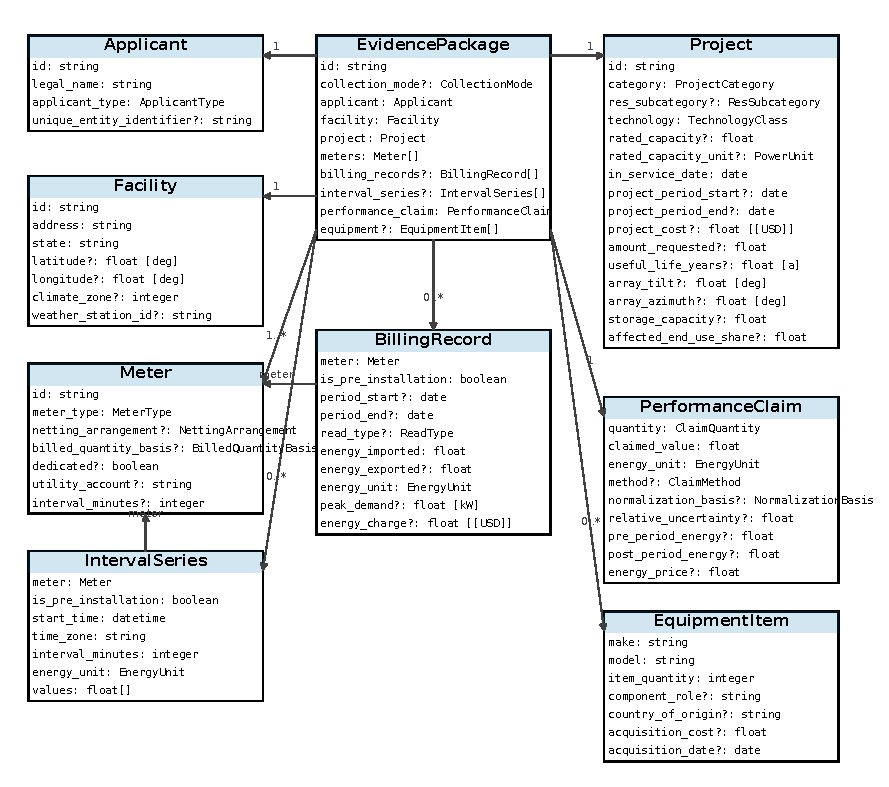
\includegraphics[width=\linewidth]{figures/fig1_schema}
\caption{Classes of the evidence schema, generated from the LinkML source. A question mark
denotes an optional element; brackets denote a list or a UCUM unit. No data are
shown.}\label{fig:schema}
\end{figure}

\subsection{Synthetic applicant generator}

Each synthetic applicant (Fig.~\ref{fig:generator}) is a facility at one of \NStates{}
hypothetical rural sites, one per State. Hourly load is
\begin{equation}
L_{\mathrm{cf}}(t)=A\Big[\sum_e o_e(t)\,b_e(t)+\sum_r c_r(t)\,\big[\pm(T(t)-T_r)\big]^{+}\Big]
\varepsilon_{\mathrm{day}}(t)\,\varepsilon_{\mathrm{hour}}(t),
\label{eq:load}
\end{equation}
with end-use shapes $b_e$ and temperature responses $c_r$ fitted to the State aggregates
of NREL's ComStock end-use load profiles \cite{wilson2022enduse,wilson2021enduse_data}
for four commercial building types, or taken from stated hypothetical shapes for
irrigation, grain-drying and dairy facilities, which the profiles do not cover;
$o_e$ represents a non-routine change in base load and $\varepsilon$ multiplicative
noise. Weather is the actual sequence of 2005--2015: irradiance from the National Solar
Radiation Database \cite{sengupta2018national} as distributed by PVGIS
\cite{huld2012new,pvgis_api}, site temperature from reanalysis, and, for the verifier's
degree days, the nearest Integrated Surface Database station
\cite{smith2011integrated} (median distance \MedianStationDistance{}~km). Pre- and
post-installation periods are consecutive, so their weather differs as it would in
practice.

A project is a photovoltaic system simulated with the PVWatts formulation
\cite{dobos2014pvwatts} in pvlib \cite{holmgren2018pvlib}, with system-specific derating,
or an efficiency measure that reduces specified end uses from the in-service day
(\ResShareAwards\% of projects are RES, the share among fiscal year 2021--2023 awards
\cite{usaspending10868}; project size is resampled from fiscal year 2021--2022 award
amounts). Utility bills follow scheduled read cycles with jitter, estimated reads that
are trued up at the next actual read, and netting of exports according to the metering
arrangement. Ground truth is retained: production $P^\ast$ in the twelve months after
$D$, pre-installation use $C^\ast$, and normal-year savings $S^\ast$, the mean annual
difference between counterfactual and actual load over the weather record.

One of six reporting errors is injected with scenario probabilities
(\CfgRateUnit--\CfgRateTransposed\% each; \ErrorShare\% of applicants in total): unit
errors, transposed digits, bills from the wrong period, a second meter counted in
pre-installation use, exports or bill reductions reported as production, and nameplate
capacity times peak sun hours reported as production. The classes follow the audit
findings and the measurement literature; the rates are hypothetical and are not estimates
of prevalence.

\begin{figure}[t]
\centering
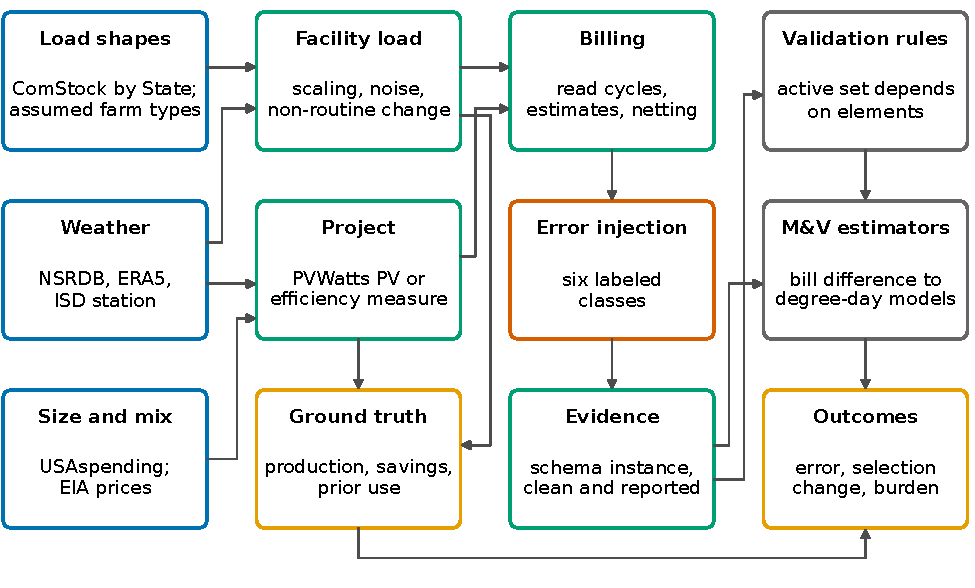
\includegraphics[width=\linewidth]{figures/fig2_generator}
\caption{Synthetic applicant generator and evaluation pipeline. All applicant data are
synthetic.}\label{fig:generator}
\end{figure}

\subsection{Estimators}

For EEI projects the rule's definition of simple payback subtracts actual from historical
energy use; we call this the undated difference, $\sum_{m\in\mathrm{pre}}E_m-
\sum_{m\in\mathrm{post}}E_m$ over twelve bills each. With billing dates the difference
can be day-annualized. With dates and a weather station, a baseline model
\begin{equation}
E_m=\beta_0 d_m+\beta_H\,\mathrm{HDD}_m(T_H)+\beta_C\,\mathrm{CDD}_m(T_C)+\varepsilon_m
\label{eq:dd}
\end{equation}
is fitted by weighted least squares on average daily use, with balance points chosen on
the CalTRACK grid by adjusted $R^2$ and non-positive slopes rejected
\cite{caltrack2methods}. Normalized annual savings are the difference between the
baseline and reporting-period models evaluated with long-term mean degree days. We use a
guarded form: normalization is applied only when both models have CV(RMSE) of at most
\CfgCvrmseMax\%; otherwise the dated difference is kept. With read type, an estimated
read is merged with the following period. With interval data the same model is fitted to
daily energy with a weekday term. Uncertainty is computed with the fractional savings
uncertainty approximation of ASHRAE Guideline 14 with an autocorrelation correction
\cite{ashrae2014guideline14,reddy2000uncertainty} and with a residual block bootstrap
\cite{kunsch1989jackknife}.

For RES projects the verified production is the applicant's annual claim, the sum of
monthly production-meter readings, or the interval total, depending on what is
collected. A plausibility statistic compares production with modelled yield for the
rated capacity and location,
\begin{equation}
z=\ln\!\big(\hat P/\hat P_{\mathrm{model}}\big)/\sigma ,
\label{eq:z}
\end{equation}
and weather-normalized production is $\hat P\,Y_{\mathrm{normal}}/Y_{\mathrm{actual}}$.

\subsection{Validation rules}

\NRules{} rules (Table~\ref{tab:rules}) check ranges, sums and recomputations, billing
continuity and alignment with the in-service date, account identity, price consistency,
export consistency, end-use bounds, payback plausibility, and statistical agreement of
claimed production with modelled yield and with the change in utility bills. Each rule
declares the optional elements it needs. Thresholds of statistical rules are set to a
\StatRuleFpr\% false-positive rate on error-free submissions. A flagged erroneous
submission is assumed to be corrected on resubmission; a flagged error-free submission
costs rework time.

\subsection{Burden model and optimization}

Respondent time for the evidence under specification $\mathbf{x}$ is
\begin{equation}
B(\mathbf{x})=\kappa\Big[\sum_{c} w_c\Big(b_c+\sum_j \tau_{jc}x_j\Big)+\phi(\mathbf{x})\,
\tau_{\mathrm{rework}}\Big],
\label{eq:burden}
\end{equation}
with $w_c$ the RES/EEI mix, $b_c$ the time for the evidence the rule already requires,
$\phi$ the flag rate and $\tau$ triangular scenario distributions. No element-level time
data exist for this collection; $\kappa$ scales the current specification to
\AnchorResponses{} responses of the published average of \AuditHoursPerResponse{} hours,
which fixes the unit without affecting the ordering of specifications. In file-based
modes a billing-history file replaces locating and typing bills.

The accuracy loss is
\begin{equation}
\mathcal{L}_1(\mathbf{x})=\frac1N\sum_n \min\!\left(\frac{|V_n(\mathbf{x})-V_n^\ast|}{|V_n^\ast|},1\right),
\label{eq:loss}
\end{equation}
with $V^\ast=P^\ast$ for RES and $S^\ast$ for EEI; the cap bounds the influence of gross
errors. The selection loss $\mathcal{L}_2$ is the mean share of applications selected on
true values that are not selected on verified values, in \NCompetitions{} simulated
competitions of \NCompetitionApplicants{} applicants scored with \S4280.140(d)(2), (3)
and (6) and selected under \S4280.150 (reserve for requests of at most \$\SmallRequest, top
\CfgTopPerState{} per State, then rank order; funds equal to \CfgFundingRatio\% of
requests in the central scenario). With $J=\NOptionalElements\le 16$ all \NSpecs{} feasible
specifications are enumerated. As a check of the method intended for larger element
sets, a quadratic surrogate of $\mathcal{L}_1$ is minimized subject to
$\sum_j\tau_jx_j\le B$ as a mixed-integer programme with HiGHS
\cite{huangfu2018parallelizing} and the solution is evaluated by simulation.

\section{Results}

Results are reported at four levels of evidence. \emph{Numerical correctness}: unit and
property tests cover energy conservation in billing, recovery of known regression
coefficients, agreement with an independent weighted least-squares implementation, the
selection invariants and the optimizer. \emph{Model verification}: the photovoltaic
model reproduces an independent PVWatts v8 run on identical hourly weather within
\PvRefAnnualDiff\% for annual energy and \PvRefMonthlyMaxDiff\% for any month.
\emph{Empirical validity} is not established: no REAP microdata or open labelled
pre/post dataset was available. \emph{Regulatory applicability}: each result maps to
one of the four Paperwork Reduction Act questions on the collection (Section~4). All
figures and tables below except the burden audit rest on \NApplicants{} synthetic
applicants (\NRes{} RES, \NEei{} EEI).

\subsection{Burden audit}

The notice gives \AuditRespondents{} respondents, \AuditResponsesPerRespondent{}
responses per respondent, \AuditResponses{} responses, \AuditHoursPerResponse{} hours per
response and \AuditTotalHours{} hours (Table~\ref{tab:audit}). The factors do not
reproduce the totals: respondents times responses per respondent is
\AuditProductResponses, and responses times hours per response is \AuditProductHours,
\AuditHoursDiscrepancy{} hours (\AuditHoursDiscrepancyPct\%) below the published total.
The published ratios are the exact ratios truncated, not rounded, to two decimals
(\AuditImpliedResponsesPerRespondent{} and \AuditImpliedHoursPerResponse). Relative to
the current inventory of \InvResponses{} responses and \InvHours{} hours
\cite{omb05700067}, responses rise \ChangeResponsesPct\% while hours fall
\ChangeHoursPct\% and respondents fall \ChangeRespondentsPct\%: responses per respondent
increase by a factor of \ChangeResponsesPerRespondentFactor{} and hours per response fall
\ChangeHoursPerResponsePct\%. The notice describes the respondents as nonprofit
corporations and institutions of higher education, whereas its abstract and the rule
address agricultural producers and rural small businesses, and it calls the request both
a revision and an extension.

\begin{table}[t]
\caption{Arithmetic of the published burden estimate (91 FR 62611) and the current OMB
inventory. Observed regulatory data; no synthetic data.}\label{tab:audit}
\centering\footnotesize
\begin{tabular}{p{0.42\linewidth}rp{0.36\linewidth}}
\hline
Quantity & Value & Basis \\
\hline
Respondents & 2{,}977 & published \\
Responses per respondent & 37.64 & published \\
Responses & 112{,}073 & published \\
Hours per response & 1.34 & published \\
Total annual hours & 150{,}883 & published \\
Respondents $\times$ responses per respondent & 112{,}054 & 19 below published responses \\
Responses $\times$ hours per response & 150{,}178 & 705 hours below published total \\
Responses $\div$ respondents & 37.6463 & rounds to 37.65; truncates to 37.64 \\
Total hours $\div$ responses & 1.3463 & rounds to 1.35; truncates to 1.34 \\
Total hours $\div$ respondents & 50.7 & derived \\
Current inventory: responses & 81{,}765 & ICR 202602-0570-001 \\
Current inventory: hours & 257{,}879 & ICR 202602-0570-001 \\
Current inventory: hours per response & 3.15 & derived \\
\hline
\end{tabular}

\end{table}

\subsection{Traceability}

Of \TraceTotal{} parsed requirement paragraphs, \TraceEvidence{} call for information held
in the schema (Table~\ref{tab:trace}). Of the schema's \SchemaSlots{} elements,
\SchemaSlotsBeyondRule{} are not called for by any paragraph; they include the read type,
the weather station, interval metadata and the normalization basis of a claim. Billing
dates and the basis of the billed quantity are implied by the rule's reference to
utility bills and metering agreements but are not required as data.

\begin{table}[t]
\caption{Requirement-to-schema traceability by section of 7 CFR part 4280 subpart B
(summary; full table in the SI).}\label{tab:trace}
\centering\footnotesize
\begin{tabular}{llrrp{0.34\linewidth}}
\hline
Section & Subject & Paragraphs & Mapped & Schema classes used \\
\hline
\S4280.104 & Definitions & 10 & 10 & BillingRecord, Meter, PerformanceClaim, Project \\
\S4280.122 & Project eligibility & 171 & 46 & BillingRecord, EquipmentItem, Facility, IntervalSeries, Meter, PerformanceClaim, Project \\
\S4280.131 & Application requirements & 73 & 14 & Applicant, BillingRecord, EquipmentItem, Facility, Meter, PerformanceClaim, Project \\
\S4280.160 & Reporting requirements & 3 & 2 & EquipmentItem, PerformanceClaim \\
\hline
\end{tabular}

\end{table}

\subsection{Accuracy by specification}

For RES projects, production read from a meter is nearly exact: with error-free evidence
the median absolute relative error is \AccCurrentCleanResMedian\% (meter error only).
What matters is reporting error. Under the current specification, with injected errors
and no validation, \AccCurrentUnvalidatedResShareTen\% of RES applicants have verified
production more than 10\% from the truth; the rules that can run on the current elements
reduce this to \AccCurrentValidatedResShareTen\%, and monthly production-meter readings
to \AccProductionMeterValidatedResShareTen\% (Fig.~\ref{fig:errors}).

For EEI projects the estimator dominates. On error-free evidence the undated difference
has a median absolute relative error of \PathUndatedNormalMedian\% of normal-year savings
(5th--95th percentile \PathUndatedNormalQLow--\PathUndatedNormalQHigh\%); the dated
difference \PathDatedNormalMedian\%; guarded normalization \PathNormNormalMedian\%,
or \PathNormMergedNormalMedian\% when estimated reads are merged; and daily interval data
\PathIntervalPathNormalMedian\%. Even with interval data
\PathIntervalPathNormalShareTen\% of projects have errors above 10\%. Error depends
strongly on the savings fraction: for projects saving less than 10\% of use the median
error of the undated difference is \BandLowUndatedMedian\% and of the normalized estimate
\BandLowNormMedian\%, against \BandHighUndatedMedian\% and \BandHighNormMedian\% for
projects saving more than 20\%. All \TestsTotal{} pre-specified paired comparisons were
significant after Holm correction (\TestsRejected{} of \TestsTotal; SI), including the
advantage of interval over normalized monthly data, so the competing outcome in which
dated, normalized monthly bills match interval data did not occur; dated bills with
normalization and read type close \GapClosedPct\% of the gap in median error between the
undated difference and interval data. Pre-installation use is well determined
from twelve complete bills (median error \PathCpreUndatedMedian\% undated,
\PathCpreDatedMedian\% dated).

\begin{figure}[t]
\centering
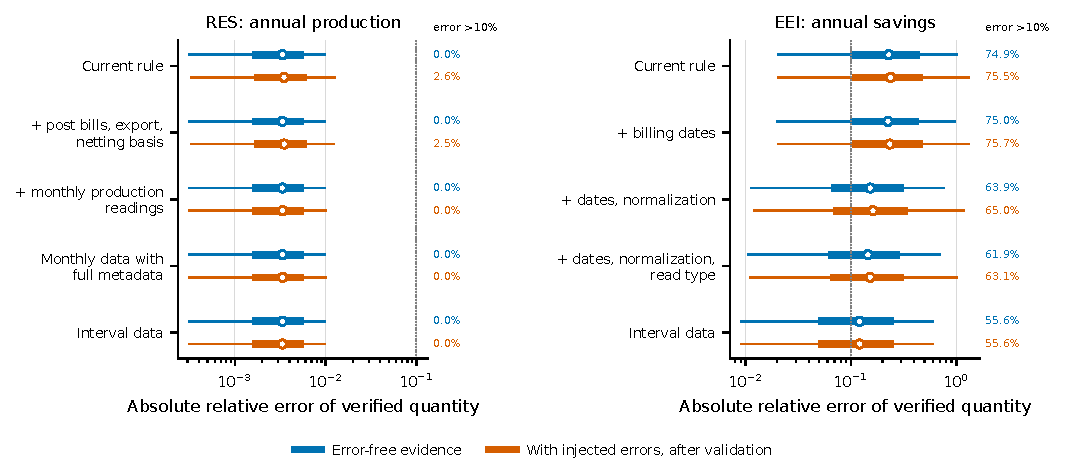
\includegraphics[width=\linewidth]{figures/fig3_error_distributions}
\caption{Synthetic data. Absolute relative error of the verified quantity by evidence
specification: median (circle), interquartile range (bar) and 5th--95th percentile
(line); numbers at right give the share of applicants with error above 10\%. Blue:
error-free evidence. Vermilion: evidence with injected errors after validation and
correction. Error-class rates are hypothetical.}\label{fig:errors}
\end{figure}

\subsection{Validation performance}

Deterministic rules detect the error class they were written for by construction
(Table~\ref{tab:rules}), so their detection rates are statements of logic, not of
measured performance: capacity-factor bounds
catch every unit error in production; date rules catch every wrong-period error;
account identifiers catch every double-counted meter; recomputation against monthly
production readings catches \DetProductionMeterResGrossNet\% of gross/net and
\DetProductionMeterResNameplate\% of nameplate claims. Without the corresponding
elements these errors are mostly invisible: under the current specification the ensemble
detects \DetCurrentResPeriod\% of wrong-period and \DetCurrentResDouble\% of
double-counting errors for RES, and \DetCurrentEeiPeriod\% and \DetCurrentEeiDouble\% for
EEI. Statistical rules are uneven (Fig.~\ref{fig:roc}). The plausibility statistic
ranks gross/net confusion (AUC \AucPlausGrossNet) and nameplate claims (AUC
\AucPlausNameplate; \AucPlausGeomNameplate{} with declared array geometry) above
error-free submissions, but at the \StatRuleFpr\% false-positive threshold it flags
\DetRulePlausGrossNet\% of the former and only \DetRulePlausNameplate\% of the latter
(\DetRulePlausGeomNameplate\% with declared geometry), because an estimate from capacity
and sun hours lies within the spread of real system performance. Comparing claimed production with the change in utility bills is weak even
when exports and the netting basis are known (AUC \AucBillDiffGrossNet{} for gross/net
confusion), because load changes between years mask the signal; and a bill-outlier rule
does not detect transposed digits (AUC \AucOutlierTransposed), most of which alter
low-order digits. Transposed digits are only partly detected in every specification
(\DetCurrentResTransposed\% for RES under the current elements and
\DetMetadataResTransposed\% with full monthly metadata), through recomputation of
totals. With
the full set of monthly metadata the ensemble recall is \DetMetadataResRecall\% (RES) and
\DetMetadataEeiRecall\% (EEI) at false-positive rates of \DetMetadataResFalsePositive\%
and \DetMetadataEeiFalsePositive\%.

\begin{table}[p]
\caption{Synthetic data. Validation rules, the optional elements they require, their
false-positive rate on error-free submissions (FP, \%) and detection rate (\%) by injected
error class: U unit, T transposed digits, P wrong period, D double counting, G gross/net,
N nameplate $\times$ hours (\NPerClass{} applicants per class). Type: dete.\ deterministic,
stat.\ statistical, diag.\ diagnostic.}\label{tab:rules}
\centering\scriptsize
\begin{tabular}{p{0.29\linewidth}p{0.15\linewidth}llrrrrrrr}
\hline
Rule & Elements required & Applies & Type & FP & U & T & P & D & G & N \\
\hline
Claimed production implies a capacity factor within bounds relative to modeled yield at the site & none & RES & dete. & 0.0 & 100 & 7 & 0 & 0 & 58 & 0 \\
Sum of production-meter readings implies a capacity factor within bounds & inverter monthly & RES & dete. & 0.0 & 100 & 0 & 0 & 0 & 0 & 0 \\
Monthly pre-installation quantities sum to the stated annual pre-installation energy & none & all & dete. & 0.0 & 0 & 11 & 0 & 0 & 0 & 0 \\
Claimed value equals the value recomputed from the submitted records & none & EEI & dete. & 0.0 & 0 & 24 & 0 & 0 & -- & -- \\
Claimed production equals the sum of production-meter readings & inverter monthly & RES & dete. & 0.0 & 0 & 32 & 0 & 0 & 99 & 98 \\
Billing periods are contiguous without gaps or overlaps & billing dates & all & dete. & 0.0 & 0 & 0 & 0 & 0 & 0 & 0 \\
Each period and the twelve-period total have a plausible number of days & billing dates & all & dete. & 0.0 & 0 & 0 & 0 & 0 & 0 & 0 \\
Pre-installation periods end before, and post-installation periods begin after, the in-service date & billing dates & all & dete. & 0.0 & 0 & 0 & 100 & 0 & 0 & 0 \\
All records come from one dedicated account in both periods & meter ids & all & dete. & 0.0 & 0 & 0 & 0 & 100 & 0 & 0 \\
Implied unit price per bill is consistent across bills and with the stated energy price & bill charges & all & dete. & 0.0 & 50 & 17 & 0 & 0 & 0 & 0 \\
No billed quantity departs sharply from its neighbours & none & all & stat. & 1.5 & 1 & 1 & 2 & 1 & 1 & 1 \\
No average daily use departs sharply from its neighbours & billing dates & all & stat. & 1.4 & 1 & 1 & 2 & 1 & 1 & 1 \\
Exports are consistent with the metering arrangement and do not exceed or equal claimed production & export channel, res post bills & RES & dete. & 0.0 & 45 & 2 & 0 & 0 & 64 & 0 \\
Claimed production agrees with the change in billed energy (billed quantity basis unknown) & res post bills & RES & stat. & 1.0 & 100 & 2 & 1 & 0 & 7 & 1 \\
Claimed production agrees with pre-installation use minus delivered energy plus exports & export channel, res post bills & RES & stat. & 1.0 & 100 & 3 & 1 & 0 & 12 & 1 \\
Claimed production agrees with modeled production for the rated capacity and location (default array geometry) & none & RES & stat. & 1.0 & 100 & 12 & 1 & 1 & 88 & 42 \\
Claimed production agrees with modeled production for the declared array geometry & pv geometry & RES & stat. & 1.0 & 100 & 13 & 1 & 1 & 89 & 60 \\
Monthly production readings follow the modeled seasonal shape & inverter monthly & RES & stat. & 1.0 & 1 & 11 & 1 & 1 & 1 & 1 \\
Savings do not exceed the share of use in the affected end uses & enduse share & EEI & dete. & 0.0 & 0 & 0 & 0 & 34 & -- & -- \\
Simple payback is neither implausibly short nor a large multiple of useful life & none & all & dete. & 1.4 & 100 & 2 & 2 & 0 & 14 & 0 \\
Baseline degree-day model meets the CV(RMSE) criterion & billing dates, weather normalization & EEI & diag. & 23.8 & 26 & 28 & 22 & 23 & -- & -- \\
\hline
\end{tabular}

\end{table}

\begin{figure}[t]
\centering
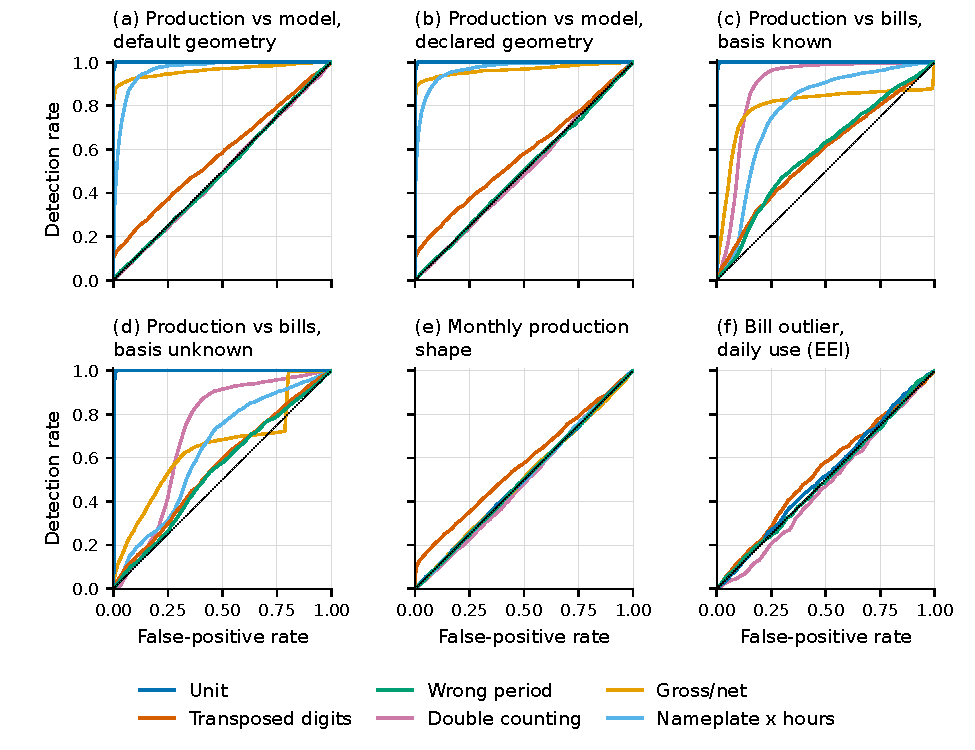
\includegraphics[width=\linewidth]{figures/fig4_validation_roc}
\caption{Synthetic data. Receiver operating characteristic of the statistical rules by
injected error class, with area under the curve in the legend.}\label{fig:roc}
\end{figure}

\subsection{Normalization}

For photovoltaic production the effect of weather is direct: the error of measured
production as an estimate of long-term production moves one-for-one with the irradiance
anomaly (slope \NormResRawSlope), with RMSE \NormResRawRmse\%; normalization by modelled
yield reduces the RMSE to \NormResNormRmse\% (Fig.~\ref{fig:norm}). The rule scores
actual production, so this matters only if the agency wants expected rather than realized
output. For EEI savings the mean bias of the unnormalized difference is small
(\NormEeiRawBias\% of pre-installation use) and its dependence on the temperature
difference between years, although statistically detectable, is slight (slope
\NormEeiRawSlope\% of use per $^\circ$C): in this population weather differences act as
noise rather than systematic bias. Normalization reduces the typical error (previous
subsection) but not the root-mean-square error: a degree-day model fitted to twelve
points occasionally fails badly, and its RMSE is \NormEeiUnguardedRmse\% of
pre-installation use unguarded and \NormEeiNormRmse\% guarded, against
\NormEeiRawRmse\% for the simple difference and \NormEeiIntervalRmse\% for interval data;
\ModelFitFailShare\% of baseline models exceed the CV(RMSE) limit. Normalization of
monthly bills therefore trades fewer moderate errors for a few larger ones. Nominal \CoverageNominal\% intervals for
avoided energy use cover the truth in \CoverageFsu\% of cases with the Guideline 14
approximation and \CoverageBootstrap\% with the block bootstrap ($n=\CoverageN$): the
former is close to nominal and the latter understates uncertainty for twelve-point
baselines.

\begin{figure}[t]
\centering
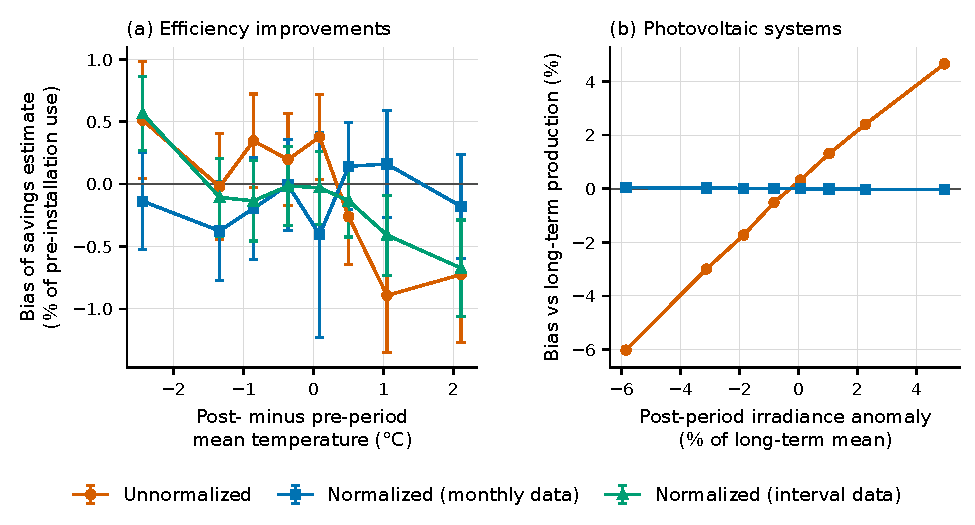
\includegraphics[width=\linewidth]{figures/fig5_normalization}
\caption{Synthetic data. Mean error of unnormalized and normalized estimates against the
weather difference between the post- and pre-installation years, with 95\% intervals of
the bin means.}\label{fig:norm}
\end{figure}

\subsection{Incomplete evidence}

When bills are missing, the undated sum understates annual use in proportion: the median
error of pre-installation use rises from \MissingZeroCpreUndated\% with complete bills to
\MissingOneCpreUndated\%, \MissingTwoCpreUndated\% and \MissingThreeCpreUndated\% with
one, two and three missing months, while day-annualization holds it to
\MissingOneCpreDated--\MissingThreeCpreDated\%; date rules flag every such case. As the
probability of an estimated read rises from \EstAProb\% to \EstDProb\%, the median error of
normalized savings rises from \EstASavNorm\% to \EstDSavNorm\% unless estimated reads are
identified and merged (\EstDSavMerged\%) (SI).

\subsection{Accuracy--burden frontier}

Fig.~\ref{fig:frontier} and Table~\ref{tab:frontier} show the frontier for manual entry.
The current specification has $\mathcal{L}_1=\BaseMare\%$ at \BaseBurden{} minutes. The
first large step is billing dates with Agency-side normalization:
\DatesNormBurdenIncrease{} minutes for a \DatesNormMareReductionPct\% reduction in loss.
Restricting attention to monthly records, the lowest-burden specification within
\RecTolerance\% of the attainable reduction collects \RecElements, at \RecBurden{} minutes
(+\RecBurdenIncreasePct\%) with $\mathcal{L}_1=\RecMare\%$ (\RecMareReductionPct\% lower)
and a flag rate of \RecFlagRate\% against \BaseFlagRate\%. Allowing interval data, the
corresponding specification (\RecIntervalElements) reaches \RecIntervalMare\% at
\RecIntervalBurden{} minutes under manual collection. Post-installation utility bills with
exports and netting basis, bill charges and a declared method do not appear on the
frontier: in this model they add checks that duplicate cheaper ones. The surrogate
programme returned optimal, feasible solutions at all \IlpNBudgets{} budgets with a
simulated loss within \IlpMaxRegret{} \pp{} of the enumeration optimum (surrogate
$R^2=\SurrogateRsq$).

\begin{figure}[t]
\centering
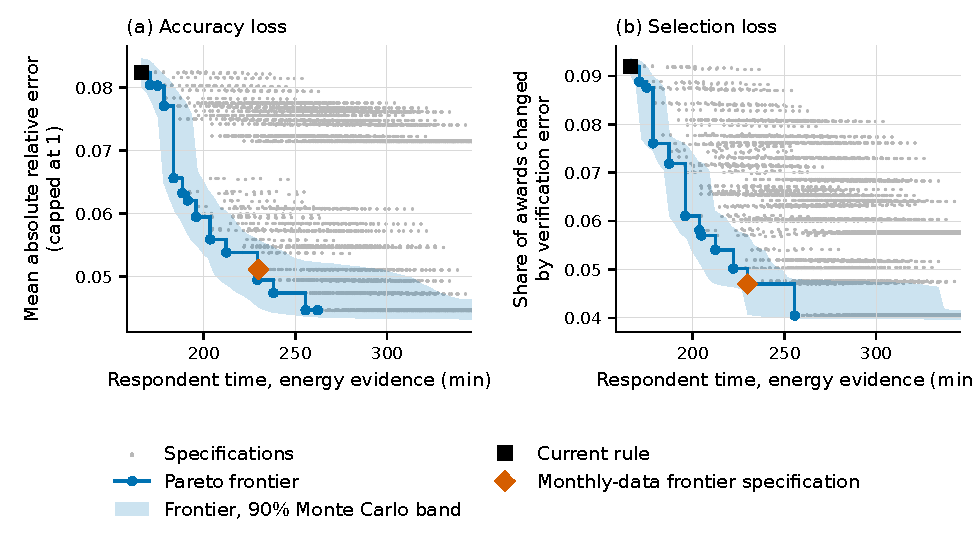
\includegraphics[width=\linewidth]{figures/fig6_frontier}
\caption{Synthetic data, hypothetical element times. Respondent time and loss of all
feasible specifications under manual entry (grey), the Pareto frontier (blue) with a 90\%
Monte Carlo band over element times and sampling error, the current rule (square) and the
selected monthly-data frontier specification (diamond). Left: accuracy loss
$\mathcal{L}_1$. Right: selection loss $\mathcal{L}_2$.}\label{fig:frontier}
\end{figure}

\begin{table}[!ht]
\caption{Synthetic data, hypothetical element times. Specifications on the accuracy
frontier under manual entry: respondent minutes, loss $\mathcal{L}_1$ overall and by
project type (\%), selection loss $\mathcal{L}_2$ (\%), share of injected errors detected
(\%) and false-positive rate (\%).}\label{tab:frontier}
\centering\scriptsize
\begin{tabular}{p{0.44\linewidth}rrrrrrr}
\hline
Optional elements collected & Min. & MARE & RES & EEI & Sel. & Det. & FP \\
\hline
(current rule) & 166 & 8.2 & 1.0 & 33.4 & 9.2 & 41 & 2.6 \\
enduse share & 171 & 8.0 & 1.0 & 32.5 & 8.9 & 42 & 2.6 \\
pv geometry & 175 & 8.0 & 0.7 & 33.4 & 8.8 & 44 & 3.1 \\
meter ids & 178 & 7.7 & 1.0 & 31.0 & 7.6 & 56 & 2.6 \\
billing dates, weather normalization & 184 & 6.6 & 1.0 & 25.9 & 7.8 & 59 & 2.9 \\
billing dates, enduse share, weather normalization & 188 & 6.3 & 1.0 & 24.8 & 7.4 & 61 & 2.9 \\
billing dates, read type, weather normalization & 191 & 6.2 & 1.0 & 24.3 & 7.5 & 59 & 2.9 \\
billing dates, meter ids, weather normalization & 196 & 5.9 & 1.0 & 23.1 & 6.1 & 75 & 2.9 \\
billing dates, read type, meter ids, weather normalization & 204 & 5.6 & 1.0 & 21.5 & 5.8 & 75 & 2.9 \\
billing dates, read type, meter ids, pv geometry, weather normalization & 212 & 5.4 & 0.7 & 21.5 & 5.4 & 78 & 3.3 \\
utility interval, weather normalization & 229 & 4.9 & 1.0 & 18.6 & 5.2 & 41 & 2.6 \\
pv geometry, utility interval, weather normalization & 238 & 4.7 & 0.7 & 18.6 & 4.8 & 44 & 3.1 \\
inverter monthly, utility interval, weather normalization & 256 & 4.5 & 0.4 & 18.6 & 4.0 & 53 & 3.3 \\
inverter interval, utility interval, weather normalization & 262 & 4.5 & 0.4 & 18.6 & 4.1 & 41 & 2.6 \\
\hline
\end{tabular}

\end{table}

\subsection{Selection effects}

In the synthetic population \ShareEnergyCap\% of applications reach the \ScoreEnergyCap-point cap of
the energy-per-dollar criterion, so competitive differences come from the banded
percentage and payback criteria and from eligibility (payback within useful life holds
for \ShareEligibleRes\% of RES and \ShareEligibleEei\% of EEI applicants on true values).
Verification error moves applications across band edges. With funds equal to
\FundRatioMid\% of requests, \SelCurrentUnvalidatedMid\% of awards differ from the
selection on true values when evidence with errors is taken at face value,
\SelCurrentValidatedMid\% after validation under the current specification, and
\SelCurrentCleanMid\% even with error-free evidence, because of estimator error alone
(Fig.~\ref{fig:selection}). The monthly-data frontier specification gives
\SelRecValidatedMid\% and interval data \SelIntervalValidatedMid\%. The share is larger
when funds are scarcer (\SelCurrentValidatedLow\% at \FundRatioLow\% of requests) and
smaller when they are ample (\SelCurrentValidatedHigh\% at \FundRatioHigh\%). Selection
is therefore sensitive, not robust, to verification error near score cut-offs, and
additional elements reduce but do not remove the sensitivity.

\begin{figure}[t]
\centering
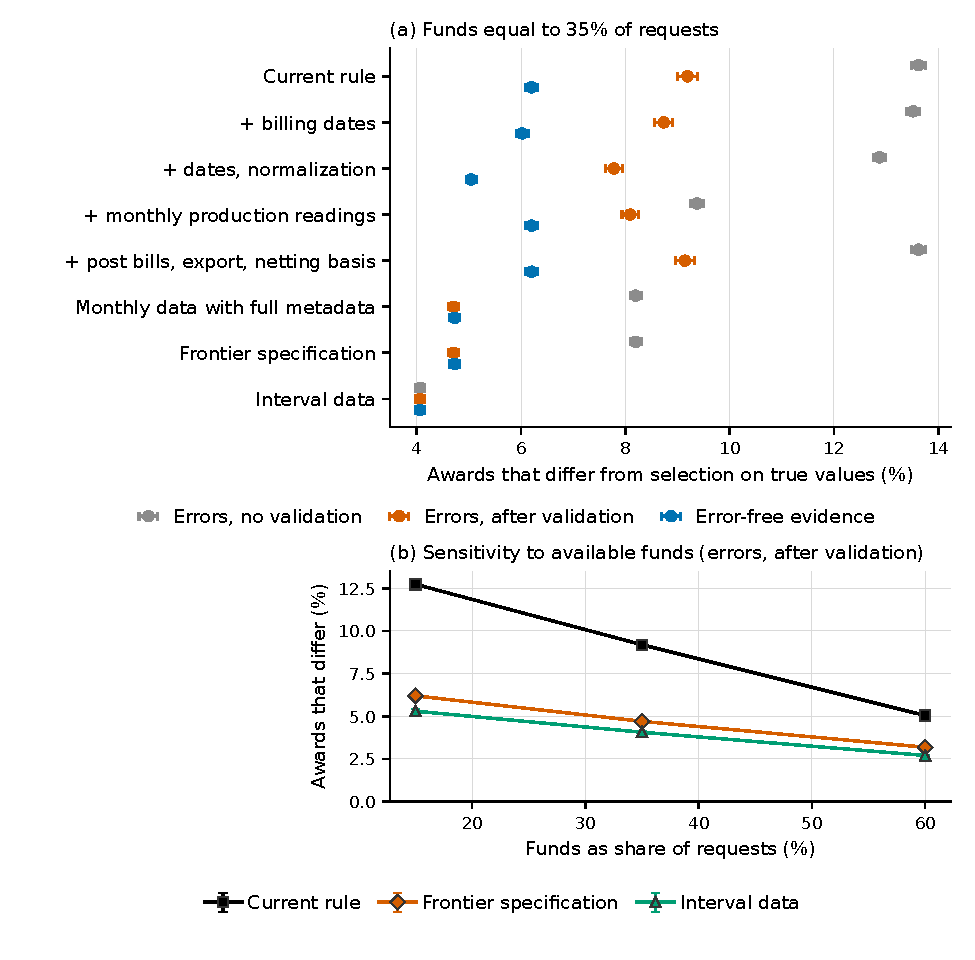
\includegraphics[width=\linewidth]{figures/fig7_selection}
\caption{Synthetic competitions with hypothetical funding and non-energy scores. Share of
awards that differ from selection on true values, by specification and condition (left,
with 95\% Monte Carlo intervals) and by available funds (right).}\label{fig:selection}
\end{figure}

\subsection{Collection modes}

If the billing history is uploaded as a utility file, the current elements take an
estimated \ModeCurrentUploadBurden{} minutes instead of \ModeCurrentManualBurden, and the
monthly-data frontier specification \ModeRecUploadBurden{} minutes
(\ModeRecUploadVsCurrentPct\% below the current manual burden) with the same accuracy,
because dates, read type and identifiers arrive with the file. With Green Button
download \cite{naesbreq21espi} or automated utility access, interval data are included
and the interval specification takes \ModeRecIntervalGreenButtonBurden{} and
\ModeRecIntervalAutomatedBurden{} minutes. These modes are not available to every
respondent; with half of respondents able to upload a file, the mean time for the
frontier specification is \ModeRecUploadHalfBurden{} minutes (SI).

\section{Discussion}

The results separate two verification problems that the rule treats alike. Production of
a metered renewable system is an observation: its accuracy is a matter of collecting the
meter record in a form that exposes reporting errors. Savings are a difference between
an observation and a counterfactual, and twelve months on each side determine them only
loosely when the measure saves a modest share of facility use. A score that bins the
percentage saved at \EeiBandEdges{} asks more precision of that
difference than the evidence holds for many projects, which is why
\SelCurrentCleanMid\% of awards change even with error-free evidence in our competitions.

For the four Paperwork Reduction Act questions, the results suggest the following,
subject to the limitations below. (a) Practical utility: the evidence as specified
supports verification of production if monthly production-meter readings are collected,
and supports only coarse verification of savings; utility would rise if the uncertainty
of savings were computed and used. (b) Burden: the published estimate cannot be
reproduced from its factors, and its respondent description does not match the program.
(c) Quality and clarity: billing dates, read type, account identifiers, array geometry and
monthly production readings are low-cost elements that enable the checks that work;
several statistical checks that sound attractive did not, and utility-side netting
information added little in this model. (d) Burden reduction: accepting billing-history files lowers time below the current
manual burden while supplying more information.

The frontier is not a single recommendation. Which point is appropriate depends on how
the agency values a percentage point of selection stability against minutes of
respondent time, a judgment the analysis informs but does not make.

\section{Limitations}

All applicants are synthetic. Load shapes for commercial buildings are State aggregates
of a calibrated stock model and are smoother than individual facilities; agricultural
shapes are assumptions and cover electricity only, whereas many REAP efficiency projects
save propane or diesel. Noise, non-routine changes, measure sizes, error-class rates,
competition size, funding and non-energy points are hypothetical; error rates in
particular are not estimates of prevalence, and the selection results depend on them.
Halving load noise and removing non-routine changes changes the median error of
the undated EEI difference from \NoiseCentralUndatedMedian\% to \NoiseLowUndatedMedian\%,
and doubling both raises it to \NoiseHighUndatedMedian\% (\NoiseLowNormMedian\%,
\NoiseCentralNormMedian\% and \NoiseHighNormMedian\% for dated, adjusted bills; SI), so the
undated result is not driven by the noise assumptions, whereas the benefit of adjustment
is. The undated median error is \BasisComstockUndatedMedian\% for ComStock-based facility
types and \BasisHypotheticalUndatedMedian\% for the hypothetical agricultural types.
Only photovoltaic RES projects are modelled. Sites cover the 50 States, not the
territories that the rule treats as States. Flagged errors are assumed to be corrected,
which is optimistic. Element times are assumptions scaled to the published average; the
Sobol analysis (SI) shows that \SobolTopName{} accounts for most of the variance of the
burden difference (total index \SobolTopST). A lognormal fit to award sizes is rejected
(Anderson--Darling \AwardFitADRes{} against a 5\% critical value of
\AwardFitADCritical), so sizes are resampled from observed awards; using the lognormal
instead changes $\mathcal{L}_1$ for the current specification from \SizeEmpCurrentMare\%
to \SizeLognCurrentMare\% in a run of \SizeSensN{} applicants. Fabricated readings are not
modelled, so the value of utility-side cross-checks as an independent source is not
measured. Empirical validity against real submissions is not established.

\section{Conclusions}

For synthetic applicants built from public load, weather and award data, twelve-month
pre/post evidence verifies photovoltaic production accurately once monthly meter readings
expose reporting errors, but verifies efficiency savings with a median error of
\PathUndatedNormalMedian\% under the rule's undated difference and
\PathNormMergedNormalMedian\% with dated bills, read type and guarded normalization.
Verification error changes \SelCurrentValidatedMid\% of awards under the current
specification. A small set of metadata elements on the accuracy--burden frontier lowers
both losses for an estimated \RecBurdenIncrease{} additional minutes under manual entry
and for less time than the current specification when billing files are accepted. The
schema, generator and analysis are reusable for other programs that award funds on
documented performance.

\section*{Data and code availability}
All code, configurations, input provenance, synthetic datasets and generated values are in
the repository \texttt{reap-reporting-schema}. No archive identifier has been assigned.

\section*{Author contributions}
Avin Gupta: conceptualization, methodology, software, validation, formal analysis, data
curation, writing, visualization.

\section*{Funding}
No funding was received for this work.

\section*{Competing interests}
The author declares no competing interests.

\bibliography{references}
\end{document}
